\documentclass[12pt]{article}
\usepackage[letterpaper, margin=1in]{geometry}
\usepackage{graphicx}
\usepackage{hyperref}
\usepackage{flafter}
\usepackage{enumitem}
\usepackage{float}
\usepackage{tabularx}
\usepackage{xspace}
\usepackage[group-separator={,}]{siunitx}
\usepackage{amsmath,amsthm,amssymb, amsthm}
\usepackage{enumitem}
\usepackage{mathtools}
\usepackage{mathptmx}
\usepackage[font=small,labelfont=bf]{caption}
\usepackage{filecontents}

\newcounter{protocol}
\newenvironment{protocol}[1]
  {\par\addvspace{\topsep}
   \noindent
   \tabularx{\linewidth}{@{} X @{}}
    \hline
    \refstepcounter{protocol}\textbf{Protocol \theprotocol} #1 \\
    \hline}
  { \\
    \hline
   \endtabularx
   \par\addvspace{\topsep}}

 \newcommand{\sbline}{\\[.5\normalbaselineskip]}% small blank line

\newcommand{\set}[1]{\left\{#1\right\}}
\newcommand{\setc}[2]{\left\{#1 \; :\; #2 \right\}}

\newcommand{\system}{stateless clients\xspace}
\newcommand{\System}{Stateless Clients\xspace}
\newcommand{\figurewidth}{0.8\textwidth}

\newcommand{\repeatcaption}[2]{%
  \renewcommand{\thefigure}{\ref{#1}}%
  \captionsetup{list=no}%
  \caption{#2 (repeated from page \pageref{#1})}%
}

\setlength{\parskip}{1em}


\begin{filecontents}{\jobname.bib}
@misc{yellowpaper,
  author = {Gavin Wood},
  title = {{Ethereum: A secure decentralised generalised transaction ledger. Byzantium version 78d7b9a.}},
  journal = {Ethereum Project Yellow Paper},
  year = {2019},
  howpublished = {\url{https://ethereum.github.io/yellowpaper/paper.pdf}}
}

@misc{bitcoin-whitepaper,
  author = {{Satoshi Nakamoto}},
  title = {{Bitcoin: A Peer-to-Peer Electronic Cash System}},
  year = {2008},
  howpublished = {\url{https://bitcoin.org/bitcoin.pdf}}
}

@misc {bitcoin,
  title = {Bitcoin},
  howpublished = {\url{https://bitcoin.org/en/}}
}

@misc {ethereum,
  title = {Ethereum},
  howpublished = {\url{https://github.com/ethereum/}}
}

@misc{visa,
  author = {Visa},
  title = {{Visa acceptance for retailers}},
  howpublished = {\url{https://usa.visa.com/run-your-business/small-business-tools/retail.html}},
  year=2018
}

@misc{cryptokitties,
  author = {Cryptokitties},
  title = {{CryptoKitties | Collect and breed digital cats!}},
  howpublished = {\url{https://www.cryptokitties.co/}},
  year=2018
}

@misc{statelessclients,
  author = {Vitalik Buterin},
  title = {{The Stateless Client Concept}},
  howpublished = {\url{https://ethresear.ch/t/the-stateless-client-concept/172}},
  year = {2017}
}

@misc{ethereumblocktime,
  title = {Ethereum (ETH) price stats and information.},
  author = {{BitInfoCharts}},
  howpublished = {\url{https://bitinfocharts.com/ethereum/}},
  year = {2019}
}

@misc{etherchain-transaction,
  title = {{Transaction details}},
  author = {{Etherchain}},
  howpublished = {\url{https://www.etherchain.org/tx/29000544fb94145da4806b4506386a2b6775d4d4abca48fec1083d646e14cd2f}}
}

@inproceedings{merkle1987digital,
  title={A digital signature based on a conventional encryption function},
  author={Merkle, Ralph C},
  booktitle={Conference on the theory and application of cryptographic techniques},
  pages={369--378},
  year={1987},
  organization={Springer}
}

@misc{rlp,
  title = {{RLP Encoding}},
  howpublished = {\url{https://github.com/ethereum/wiki/wiki/RLP}}
}

@misc{merkle-patricia-trie,
  title = {{RLP Encoding}},
  howpublished = {\url{https://github.com/ethereum/wiki/wiki/Patricia-Tree}}
}

@misc {ethereum-stateless-analysis,
  title = {{Detailed analysis of stateless client witness size, and gains from batching and multi-state roots}},
  author = {{Vitalik Buterin}},
  howpublished = {\url{https://ethresear.ch/t/862}},
  year = {2018}
}

@misc {ethereum-sharding,
  title = {{Sharding introduction R\&D compendium}},
  howpublished = {\url{https://github.com/ethereum/wiki/wiki/Sharding-introduction-R&D-compendium}}
}

@misc {solidity,
  title = {{Solidity}},
  howpublished = {\url{https://github.com/ethereum/solidity}}
}

@misc {ethash,
  title = {{Ethash}},
  howpublished = {\url{https://github.com/ethereum/wiki/wiki/Ethash}}
}

@inproceedings{androulaki2018hyperledger,
  title={{Hyperledger Fabric: A distributed operating system for permissioned blockchains}},
  author={Androulaki, Elli and Barger, Artem and Bortnikov, Vita and Cachin, Christian and Christidis, Konstantinos and De Caro, Angelo and Enyeart, David and Ferris, Christopher and Laventman, Gennady and Manevich, Yacov and others},
  booktitle={Proceedings of the Thirteenth EuroSys Conference},
  pages={30},
  year={2018},
  organization={ACM}
}

@misc {parity,
  title = {Parity Ethereum 2.2.11-stable},
  howpublished = {\url{https://github.com/paritytech/parity-ethereum/releases/tag/v2.2.11}}
}

@misc {rlpx,
  title = {{The RLPx Transport Protocol}},
  howpublished = {\url{https://github.com/ethereum/devp2p/blob/master/rlpx.md}}
}

@misc{ethereum-wire-protocol,
  title = {{Ethereum Wire Protocol (ETH)}},
  howpublished = {\url{https://github.com/ethereum/devp2p/blob/master/caps/eth.md}}
}

@misc{ethereum-cross-shard,
  title = {{Ethereum Sharding FAQ}},
  howpublished = {\url{https://github.com/ethereum/wiki/wiki/Sharding-FAQ#how-can-we-facilitate-cross-shard-communication}}
}

@misc{vitalik-interview,
  title = {{Crypto Bites: Chat with Ethereum founder Vitalik Buterin}},
  year = {2019},
  howpublished = {\url{https://www.youtube.com/watch?v=u-i_mTwL-FI}}
}

\end{filecontents}

\title{Implementing \System in Ethereum}
\author{Souvik Banerjee}
\date{}

\begin{document}

\maketitle
\thispagestyle{empty}

\begin{center}
  \textsc{\textbf{Abstract}}
\end{center}

Ethereum is a blockchain based cryptocurrency and platform for decentralized applications. A key problem that Ethereum currently faces is scalability. Ethereum can only process about 15 transactions per second, while other payment processors like Visa can process \num{24000} transactions per second.  One reason for these scalability problems is due to disk I/O operations. \emph{\System} is a proposal to improve the scalability of Ethereum by reducing the amount of I/O operations Ethereum nodes need to perform. The \System proposal does this by using Merkle proofs of state values accessed during transaction execution. These Merkle proofs are called \emph{witnesses}. Witnesses are created and sent along with transactions in blocks from miners to other Ethereum nodes. Ethereum nodes use witnesses to verify transactions without needing access to the Ethereum state, which greatly reduces the amount of I/O operations. However, a major problem with this proposal is that the size of the witnesses is extremely large, which makes using \System impractical. In this paper, I show how \System works in detail, discuss how I implemented \System in the Parity Ethereum client, and present results that demonstrate that the \System proposal is not practical.

\par\bigskip\noindent\vspace{1.5in}
\begin{center}
  Advisor: Vijay Chidambaram \\
  Second Reader: Chris Rossbach \\
  Third Reader: Alan K. Cline \\
\end{center}

\newpage

\tableofcontents
\newpage


\section{Introduction} \label{section:introduction}

% reword first two sentences

In the last few years, blockchain technology has become increasingly popular.
Blockchain is a decentralized data sharing technology that works in a distributed environment consisting of multiple nodes. It can be defined as an immutable \emph{ledger} that records transactions. The blockchain structure consists of cryptographically signed \emph{blocks} that are linked to each other with cryptographic hashes. Each block contains \emph{transactions} that show value transfers between different accounts. Each node in the network maintains its own copy of the blockchain, which makes the ledger a \emph{distributed ledger}. The ledger is kept up to date using a distributed consensus mechanism, which allows nodes to validate transactions, package them into blocks, and update the block hash chain.

Blockchain and cryptocurrency are two different concepts, but their development has been intertwined. Blockchain was first suggested by Satoshi Nakamoto's paper introducing Bitcoin~\cite{bitcoin} in late 2008. Bitcoin is a cryptocurrency and is a specific implementation of blockchain technology.

Ethereum~\cite{ethereum} is a cryptocurrency that builds upon the ideas introduced in Bitcoin. Ethereum is a transaction-based state machine that starts with some initial \emph{genesis} state, incrementally executes transactions, and arrives at a final state. These transactions are collected into blocks, and blocks are hashed to create a hash chain. The Ethereum protocol has a native currency called Ether and is abbreviated as ETH.

The goal of Ethereum is to create a platform for decentralized applications, and it does this by incorporating a built-in Turing complete programming language. This allows users to write \emph{smart contracts} that contain arbitrary code and run on the decentralized Ethereum network. In contrast to Bitcoin, where transactions are simply value transfers between accounts, Ethereum transactions can create and run smart contracts. The ability to run arbitrary code makes Ethereum an extremely powerful abstraction layer on which decentralized applications can be built.

One problem with blockchain-based systems is that they are orders of magnitude slower than their centralized equivalent. Ethereum is only able to process about 15 transactions per second~\cite{vitalik-interview}, while payment processors like Visa can process \num{24000} transactions per second~\cite{visa}. New distributed applications that run on Ethereum such as CryptoKitties~\cite{cryptokitties} have slowed down transaction processing time even further. Improving the scalability of blockchain-based systems is crucial for widespread adoption.

A proposed solution to Ethereum's scalability problems is called \emph{\System}~\cite{statelessclients}. \System was proposed by Vitalik Buterin, the founder of Ethereum, in 2017. \System aims to improve scalability by reducing I/O when verifying blocks. However, until now there has been no working prototype of \System.

The structure of this paper is as follows: first, I will review some foundational concepts in Ethereum. Second, I will describe in more detail how \System is designed and how I implemented \System in Parity~\cite{parity}. Third, I will show some of the results I obtained from my implementation.

\section{Background}

\subsection{Ethereum Virtual Machine}

Ethereum is a platform for deploying and running smart contracts~\cite{yellowpaper}. Smart contracts are programs that enforce a contract and run on the Ethereum Virtual Machine, or EVM. Smart contracts are created with the \emph{Solidity} programming language and compile to EVM opcodes~\cite{solidity}. The Ethereum blockchain is replicated on many nodes and all nodes verify the correct execution of the smart contract. This makes smart contracts useful for self-executing agreements between two parties.

These EVM opcodes allow the EVM to be Turing complete, limited only by the following factors:
\begin{enumerate}
  \item Stack space: The stack has a capacity of 1024 entries, and each entry is 256 bits. The EVM is a stack-based virtual machine and the stack is used to push arguments to opcodes.
  \item Execution time: Ethereum measures ``computational effort'' using \emph{gas}. Each opcode in a contract requires a certain amount of gas to pay for its execution. Contracts run as part of transactions, and one field in the transaction is called the \emph{gas price}. In order to pay for a contract's execution, the amount of gas consumed during the execution is multiplied by the gas price, and the resulting product is deducted from the transaction sender's account.
  \item Memory: Memory is used for storing variables and calling functions. No hard limit exists on the amount of memory that may be used, but memory must be paid for with gas. The cost grows quadratically according to the following equation.
  % Equation 296 in the Yellow Paper
  \begin{align*}
    C_{mem}(a) &\equiv G_{memory} \cdot a + \lfloor \frac{a^2}{512} \rfloor  & \text{(Equation 296 in~\cite{yellowpaper})}\\
  \end{align*}
  $G_{memory}$ is a constant defined to be $G_{memory} = 3$, and $a$ is the amount of $256$-bit words used.
  \item Storage: Contracts may also store and read data in permanent storage. The \texttt{SSTORE} opcode stores a value to contract storage. This opcode costs 5,000 gas when writing to an existing value and 20,000 gas when writing to a new value. There is no hard limit on contract storage, but it is stored on each Ethereum node and is limited by hard drive capacity. Therefore, to discourage overuse of contract storage, the gas price is very high.
\end{enumerate}



\subsection{Ethereum Transactions and Blocks}

\emph{Transactions} are how the outside world communicates with Ethereum. A transaction can either transfer ETH between two accounts, create a smart contract, or call a smart contract. A transaction has a \emph{sender} and a \emph{receiver} which are identified by account addresses.

Each account in Ethereum is identified by a 160-bit address, and accounts can either belong to smart contracts or individuals. Smart contract addresses are determined when a contract is created using metadata from the account of the contract creator (the sender of the contract create transaction). Individual accounts use public and private keys, and the account address is the rightmost 160 bits of the SHA-3 (Keccak) hash of the public key. % footnote: explain Keccak vs SHA-3???

\begin{figure}[H]
  \centering
  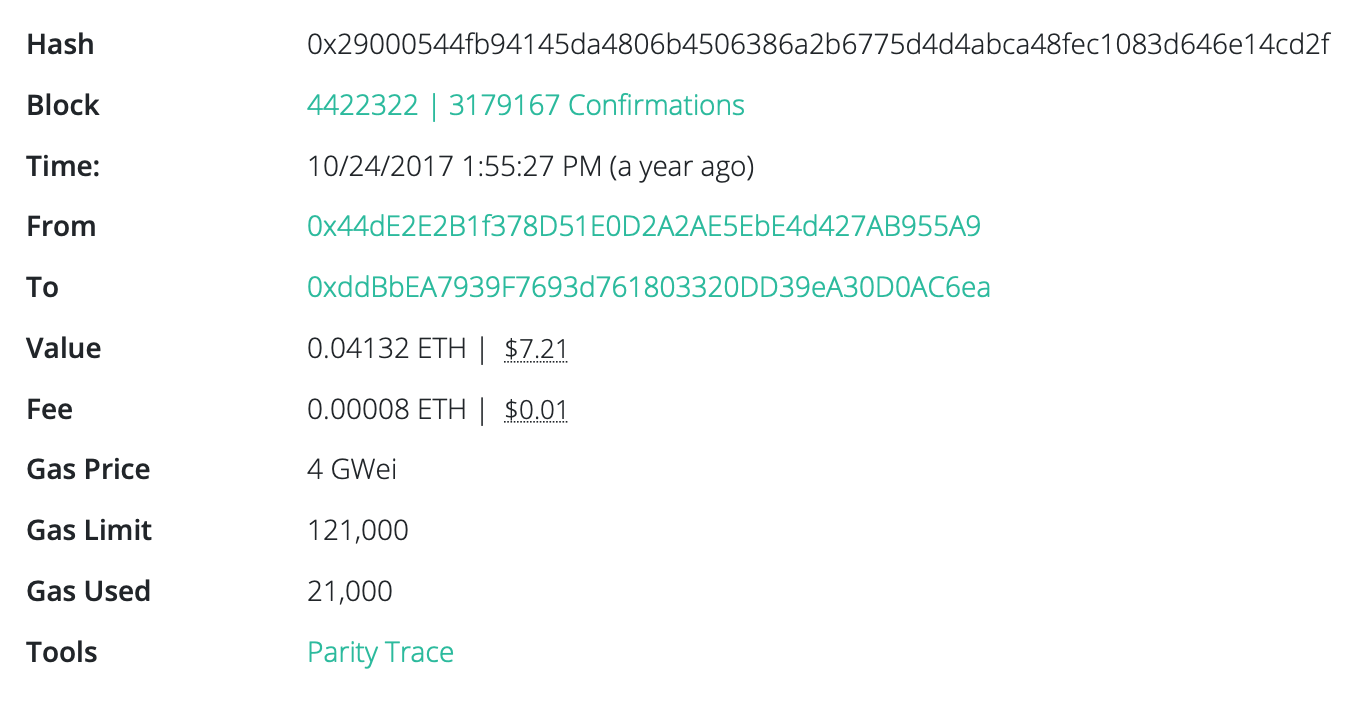
\includegraphics[width=\figurewidth]{../figures/background/transactions/example_transaction.png}
  \caption{An example transaction, with sender and receiver addresses~\cite{etherchain-transaction}. Transactions are uniquely identified by their hash. This is the SHA-3 hash of the serialized transaction (Section~\ref{subsection:rlp}).}
\end{figure}

\emph{Blocks} in Ethereum are collections of transactions. Blocks contain transactions and a \emph{header}, which contains metadata about the block. One field in the header is the \emph{parent block hash}. Blocks ``build'' on top of previous blocks by including the SHA-3 hash of the previous block in the block header. This forms a ``hash chain'' of blocks. The hash chain makes it impossible to modify previous blocks. Modifying a previous block would change the hash of the modified block and all blocks afterward.

\begin{figure}[H]
  \centering
  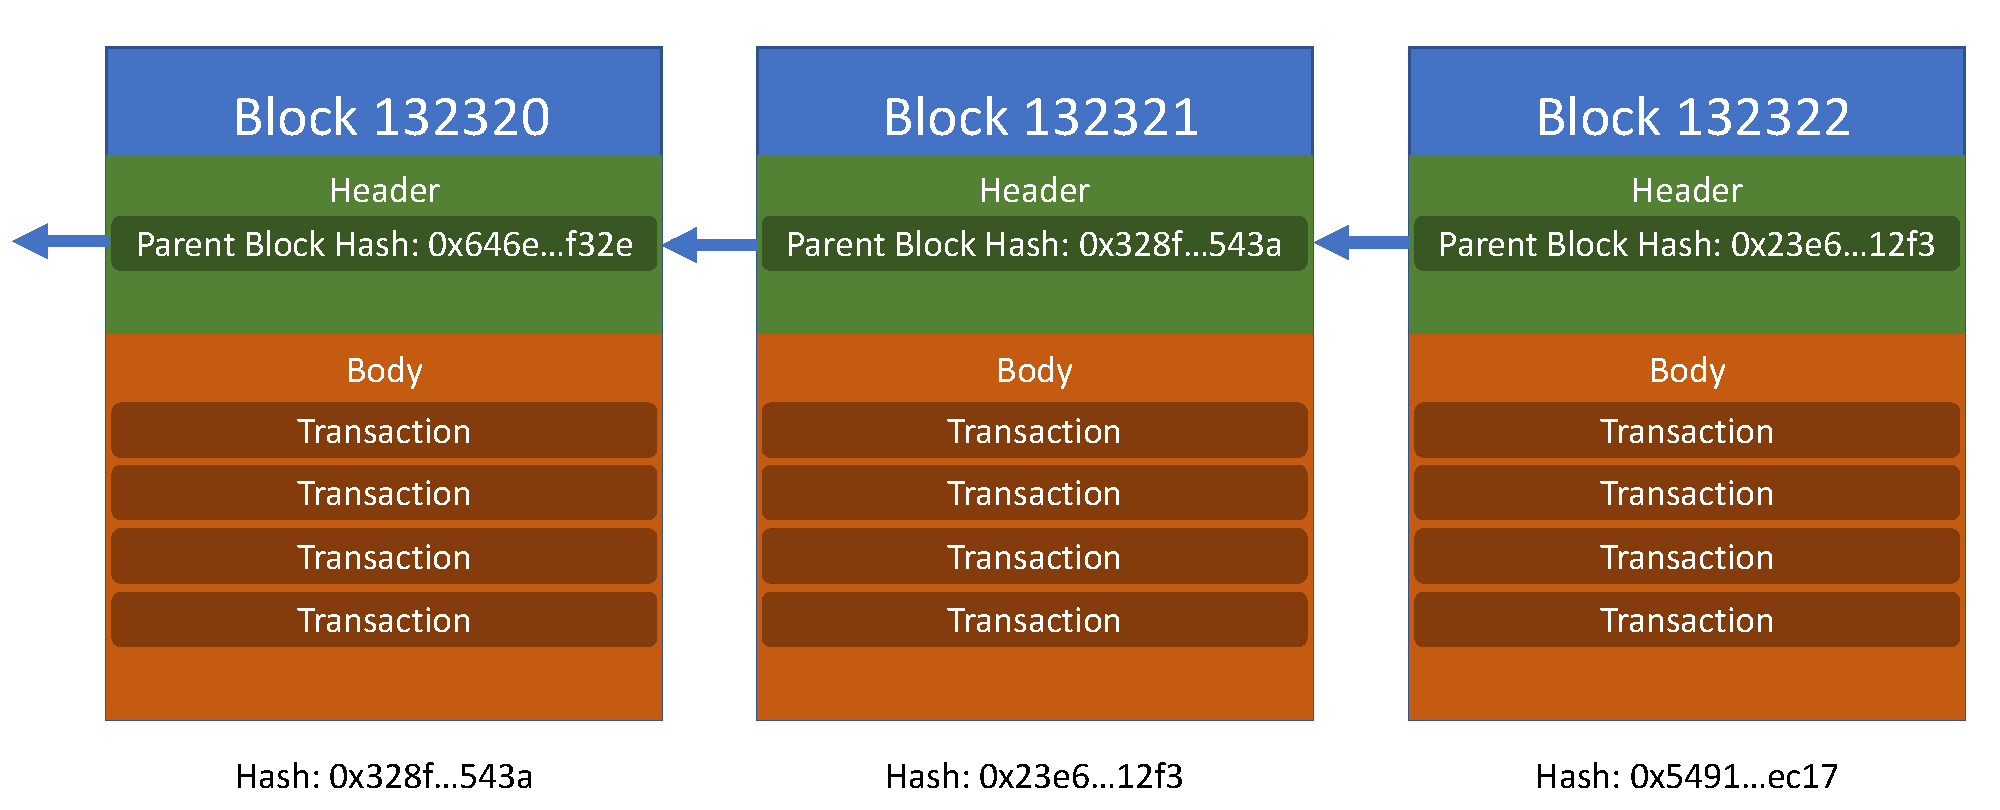
\includegraphics[width=\figurewidth]{../figures/background/blocks/blocks.pdf}
  \caption{A block hash chain with 132322 blocks; the last 3 blocks are displayed. Block hashes are shown below each block. The full hash is 256 bits, but only the first and last 16 bits are shown for brevity.}
\end{figure}


\subsection{Recursive-Length-Prefix (RLP) Encoding} \label{subsection:rlp}

Ethereum has a native serialization encoding called Recursive Length Prefix (RLP)~\cite{rlp}. RLP encodes arbitrarily nested lists of binary data. It is similar to other encoding schemes like JSON, but the range of types that are supported are limited to only lists and binary data. RLP is used to serialize blocks, transactions, and other data structures used in Ethereum.

\subsection{Merkle-Patricia Trie} \label{subsection:merklepatriciatrie}

Ethereum stores account balances and other account metadata in a data structure called a \emph{Merkle-Patricia trie}~\cite{merkle-patricia-trie}. A Merkle-Patricia trie builds upon both radix tries and Merkle trees~\cite{merkle1987digital}. Each node in the trie is hashed by first serializing with RLP, then using the SHA-3 hash function. This builds a key-value map of node hashes to nodes.

\begin{figure}[H]
  \centering
  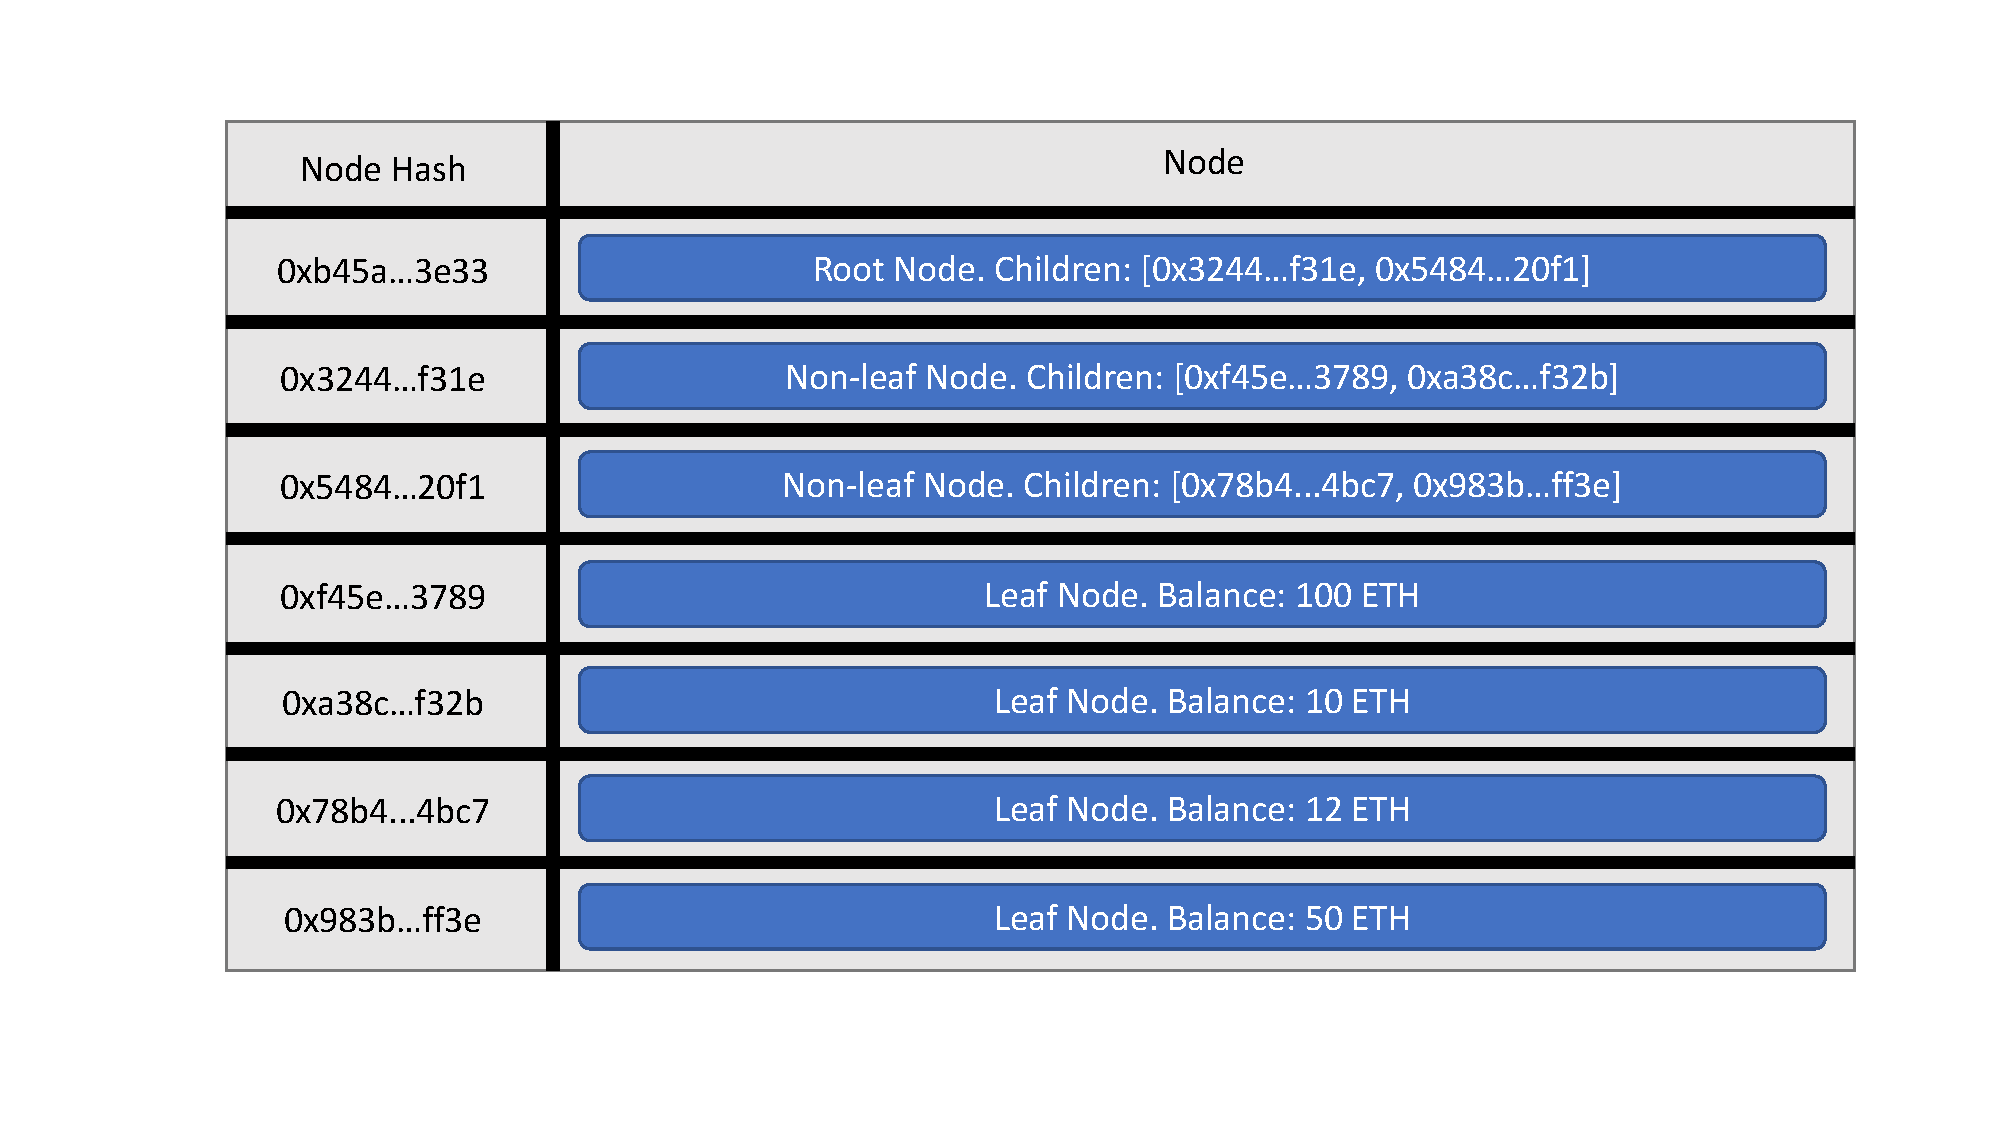
\includegraphics[width=\figurewidth]{../figures/background/trie/tree_nodes.pdf}
  \caption{Trie nodes, indexed by their hash.} \label{fig:trienodes}
\end{figure}

Nodes connect with their children by using their hash, which is stored inside the node. This makes the hash of a node depend on the hashes of its children, which are dependent on the hashes of the grandchildren, and so on. The hash of the root node can then be used to uniquely identify the entire trie.

\begin{figure}[H]
  \centering
  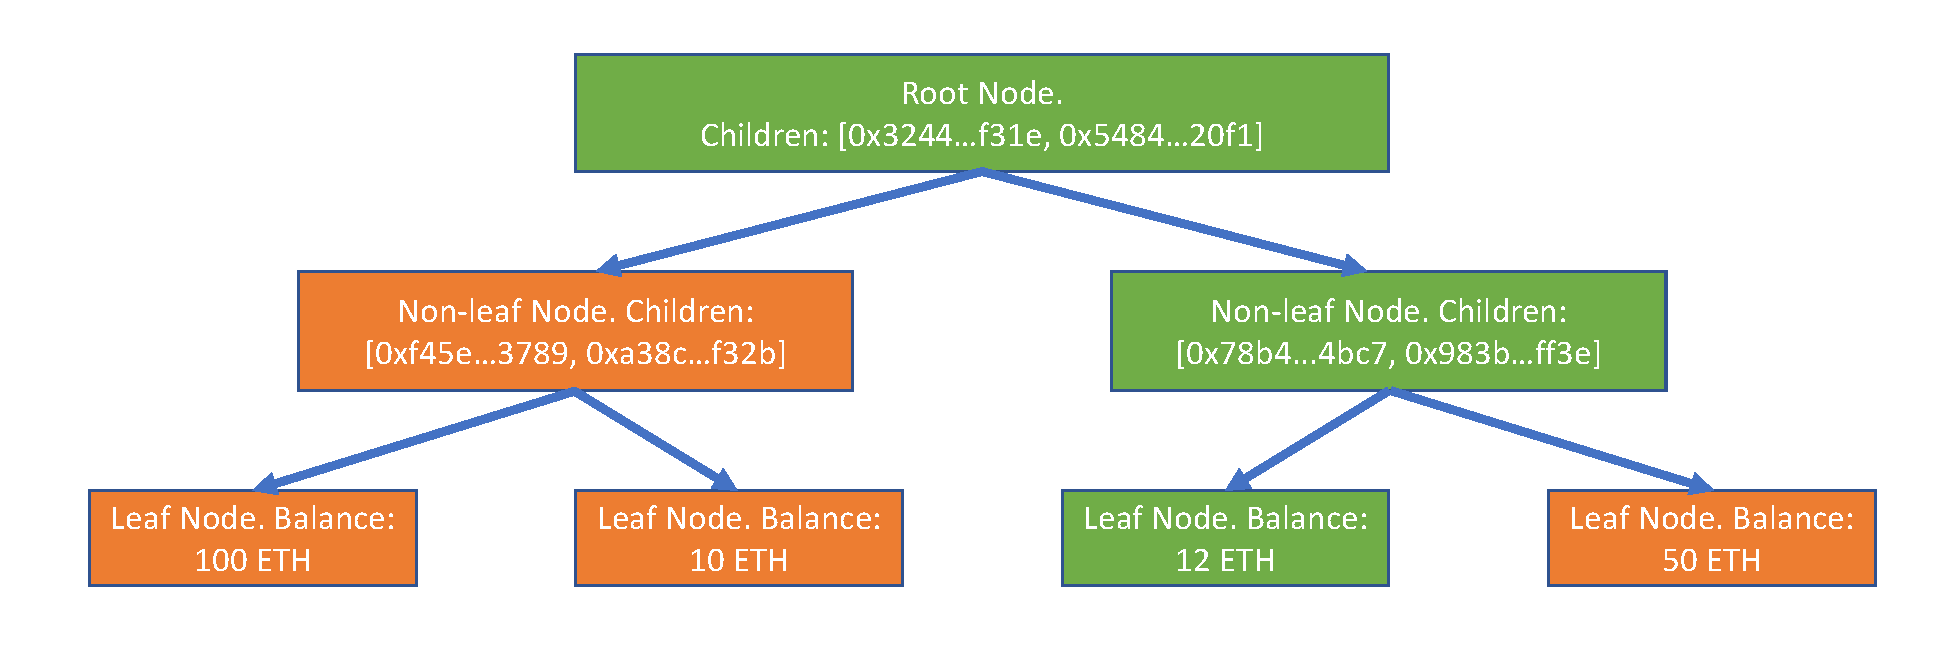
\includegraphics[width=\figurewidth]{../figures/background/trie/tree_with_merkle_proof.pdf}
  \caption{The Merkle-Patricia trie. The nodes in green represent the Merkle proof for the account with a balance of 12 ETH.} \label{fig:trie}
\end{figure}

Merkle-Patricia tries also allow one to \emph{verify} values in the trie using a \emph{Merkle proof}. A Merkle proof of a value is the set of nodes along the path to the value in the trie. If someone knows the root hash of the trie and has a Merkle proof of a value, they can verify that this value exists in the trie.


Merkle-Patricia tries are used to store the Ethereum \emph{world state}, as well as contract storage, transactions within a block, and block receipts. The Ethereum world state is the state of all accounts in Ethereum and is uniquely identified by the SHA-3 hash of the root node. Every time an account changes (for example, if the account balance changes), the hash of the root node also changes. In Figure~\ref{fig:trie}, the state root hash is \texttt{0xb45a...3e33}, as shown in Figure~\ref{fig:trienodes}.

Ethereum is a transaction-based state machine, since applying a transaction to a state $S$ produces a new state $S'$. The hash of the root node (also known as the ``state root hash'') is stored in the block header, uniquely identifying the state produced after executing the transactions in that block.

 % TODO: should I go into more detail? it is pretty complicated and would take a few paragraphs to describe fully

\subsection{Consensus} \label{subsection:consensus}
Ethereum supports multiple consensus protocols, but the protocol that is most popular is \emph{Proof-Of-Work} (PoW)~\cite{bitcoin-whitepaper}. Proof-Of-Work deters abuse by requiring that nodes perform computationally intensive tasks. This consensus protocol requires that nodes send proofs that the computationally intensive work has been done. These proofs are easy to verify but are difficult to create.

In PoW, blocks must be \emph{mined} before they are added to the hash chain. Nodes which mine blocks are called \emph{miners}. Any node in Ethereum may choose to be a miner.
Miners mine blocks by choosing values for the \emph{nonce}, a field in a block's header. A block is successfully mined if the block's hash satisfies a certain condition. By modifying the nonce field in the block header, serializing the block header with RLP, and finding the SHA-3 hash of the serialized header, we obtain the block hash. Once a nonce that satisfies the PoW condition has been found, the miner advertises the mined block on the network. Other nodes on the network verify that the block has been mined correctly by hashing the block header and checking if it satisfies the PoW condition.

Ethereum mining uses the \emph{Ethash} algorithm~\cite{ethash}. This algorithm is designed to be difficult to run on application-specific integrated circuits (ASICs) by using a significant amount of memory. Ethash uses a resource that is several gigabytes large and is regenerated every \emph{epoch transition}, which happens every 30000 blocks. This shared resource is called a DAG (directed acyclic graph) and is only needed to create the Proof-Of-Work. The DAG is not required for Proof-Of-Work verification.

Miners in Ethereum are rewarded by a predetermined block reward and by the transaction fees from the transactions they include in the block. Reward distribution is done by including the account address of the miner in the block's header. This is called the block's \emph{coinbase}. Miners also do not coordinate mining blocks and race against each other to mine the next block in the block chain. Since there is no coordination, it is possible for more than one block to be generated simultaneously. If this happens, then one block will be chosen to be added onto the main block chain, and the other blocks become \emph{uncle blocks}. Miners are still rewarded for producing uncle blocks, but the reward is not as high as for producing a normal block.

% sources:
% https://www.investinblockchain.com/vitalik-ethereum-needs-100k-transactions-per-second/
% https://www.bbc.com/news/technology-42237162

\section{Design}

\subsection{Motivation}

% Use RainBlock motivation/background for inspiration

Ethereum currently suffers from scalability problems. As stated in section~\ref{section:introduction}, Ethereum can only support about 15 transactions per second which is too slow for widespread adoption. One reason for the lack of scalability is I/O. The amount of I/O nodes need to perform is significant and slows down transaction processing. Disk I/O has also been a source of denial-of-service (DoS) attacks in Ethereum~\cite{statelessclients}. Most of these I/O operations come from traversing and updating the Merkle-Patricia trie storing the Ethereum world state. Making matters worse, the way Merkle-Patricia tries are stored on disk causes pointer-chasing random disk reads. Merkle-Patricia tries are typically stored in key-value stores such as LevelDB or RocksDB, where each value is stored using the SHA-3 hash of the value as the key. This randomizes the location of state trie nodes on disk.

\begin{figure}[H]
  \centering
  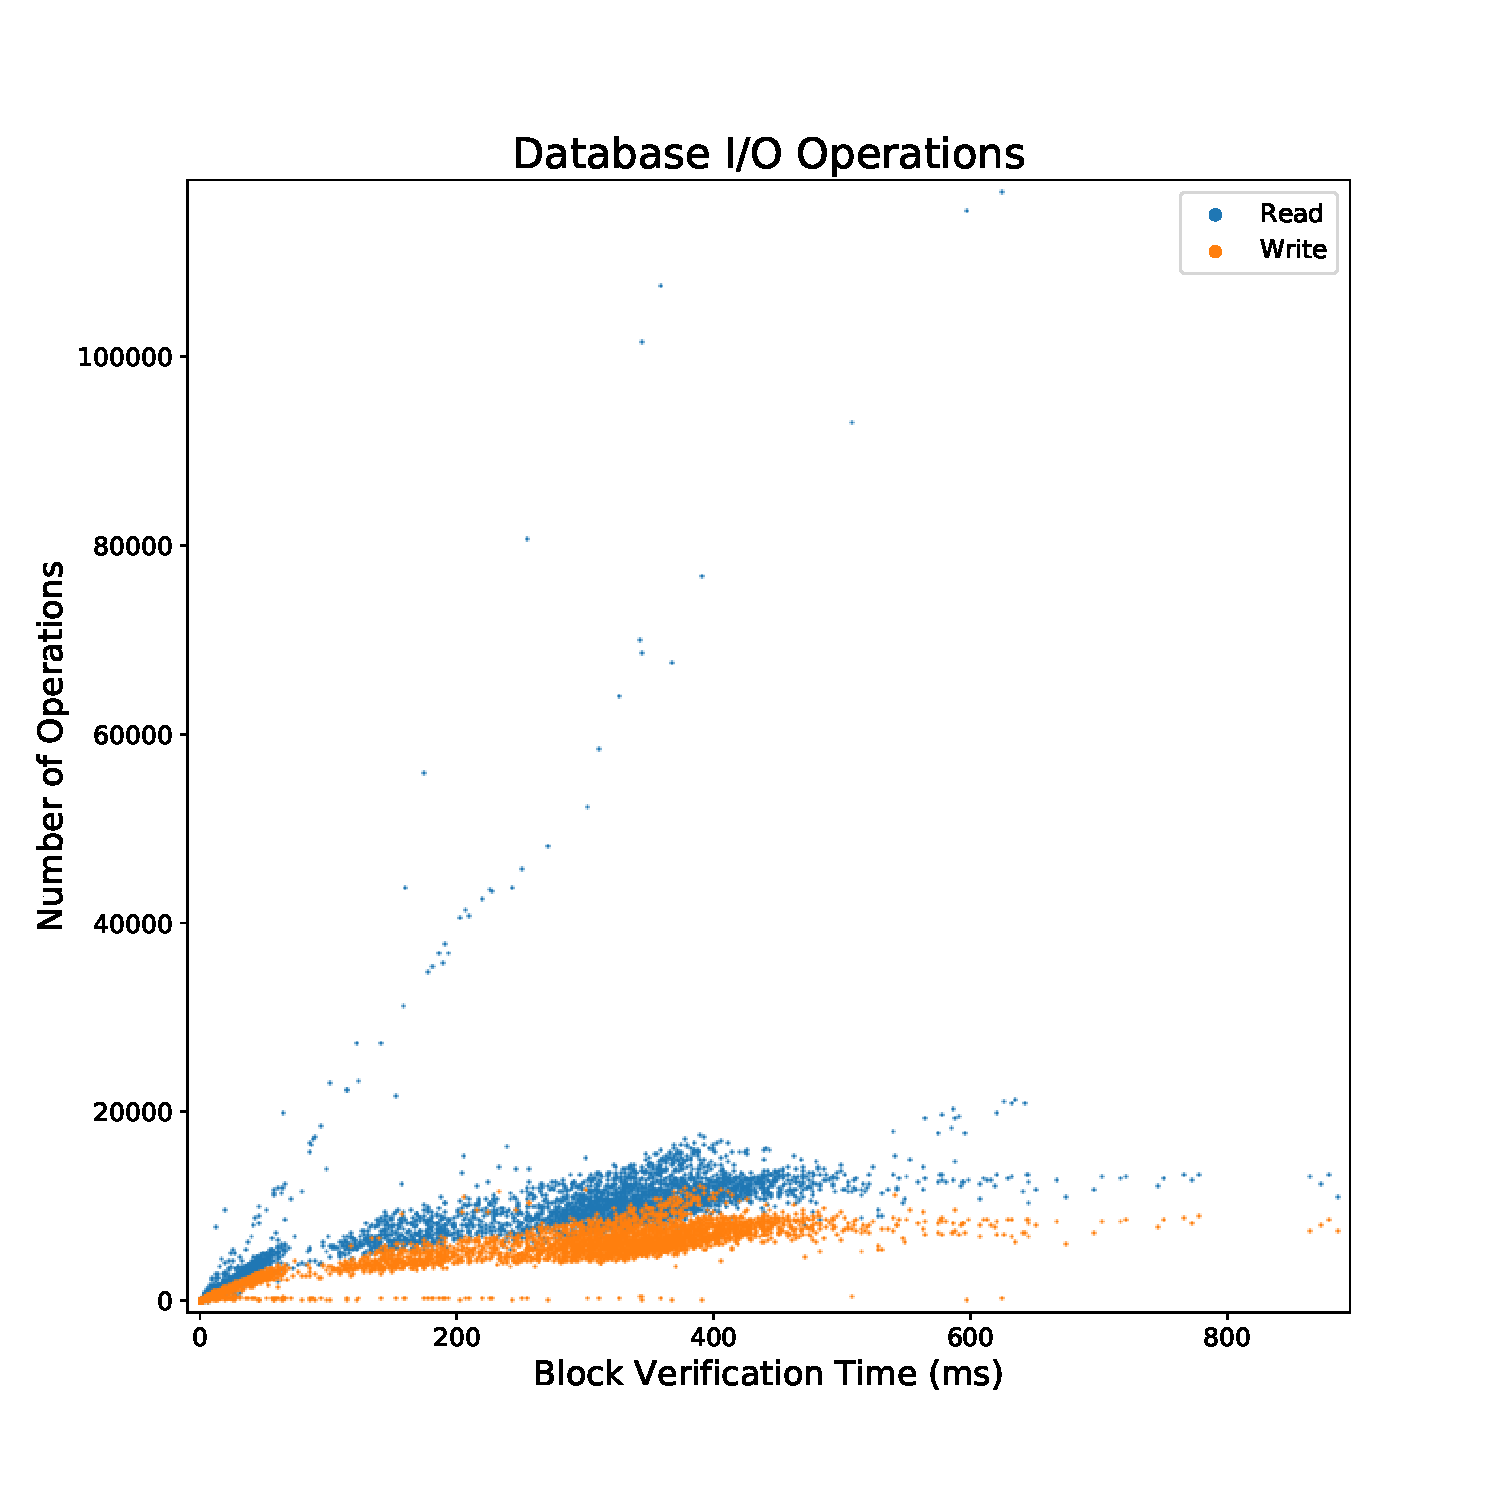
\includegraphics[width=\figurewidth]{../figures/results/graphs/background/db-io-ops-elapsed.pdf}
  \caption{I/O Operations vs. block verification time. There is a positive correlation between the amount of I/O operations performed during block verification and block verification time.}
  \label{fig:blockverificationtime}
\end{figure}

\begin{figure}[H]
  \centering
  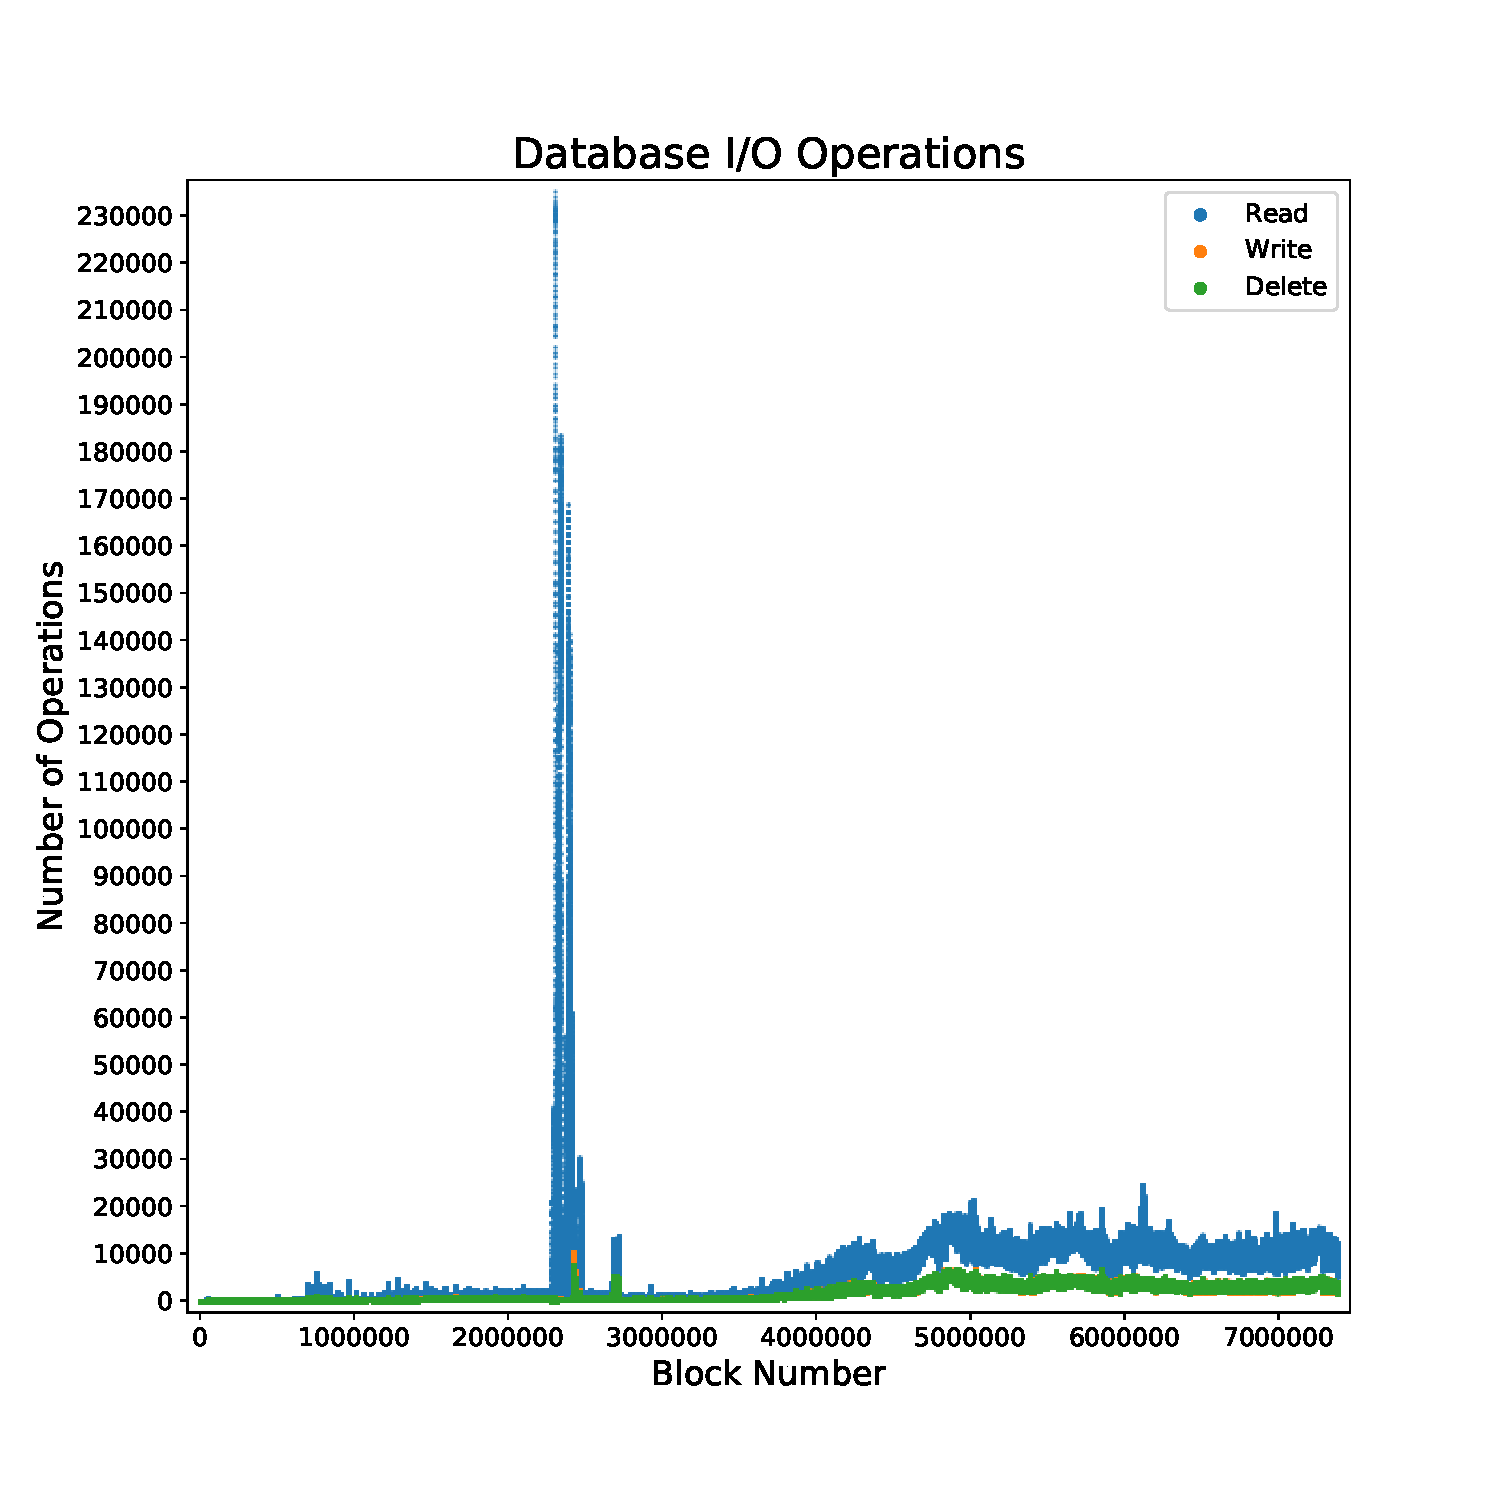
\includegraphics[width=\figurewidth]{../figures/results/graphs/background/db-io-ops.pdf}
  \caption{I/O operations performed during block verification}
  \label{fig:blockverification}
\end{figure}

Figure~\ref{fig:blockverificationtime} shows that the number of I/O operations is correlated with how long it takes to verify a block. In Figure~\ref{fig:blockverification}, the number of I/O operations is also increasing with block number. This means that the number of I/O operations will continue to increase in the future, further slowing down block verification time and affecting the scalability of Ethereum.

\subsection{\System}

The \System proposal, as the name suggests, changes Ethereum such that Ethereum nodes no longer need to store the Merkle-Patricia trie storing the Ethereum state. The term ``client'' is a synonym for ``node''. The proposal accomplishes this by changing the Ethereum state transition function. The original Ethereum state transition function is the following:
\begin{align*}
  STF(S, B) &\to S'
\end{align*}
Here, $S$ is the initial state, $B$ is an Ethereum block, and $S'$ is the new updated state created from applying the transactions in $B$ to $S$.

The \System proposal changes the state transition function to $STF'$, which is defined here:
\begin{align*}
  STF'(r_S, B, W) \to r_{S'}
\end{align*}
Here, $r_S$ is the state root hash for $S$, $B$ is a block, and $r_{S'}$ is the state root hash for $S'$. $W$ is a ``witness'', which are Merkle proofs for each value in the state trie the execution of $B$ needs to access. These witnesses are packaged along with blocks and are sent over the network to other Ethereum nodes. Since witnesses contain the state values the execution of $B$ requires, Ethereum nodes do not need to access the state trie when verifying blocks. Not having a state trie greatly reduces the number of I/O operations needed to verify blocks.

The only nodes that need to access the state trie are miners. In vanilla Ethereum, miners create blocks by including transactions and performing the Proof-Of-Work algorithm. The \System proposal adds an additional step: generate the witness for the block. Miners need to execute the transactions in the block using their local copy of the Ethereum state trie and keep track of which state values were accessed to obtain Merkle proofs. The set of Merkle proofs is the witness for the block.

\subsection{Example}

In this section, I will show how the \System proposal works from block creation to block verification using an example Merkle-Patricia trie and transaction.

\subsubsection{Block creation}

The initial Merkle-Patricia state trie is shown in Figure~\ref{fig:example:initial}. This trie contains 22 Ethereum accounts. Four accounts are shown, specifically accounts \texttt{0x1354\ldots f78b}, \texttt{0x298a\ldots e2b1}, \texttt{0x737b\ldots fc91}, \texttt{0xa98b\ldots 3645}.
\begin{figure}[H]
  \centering
  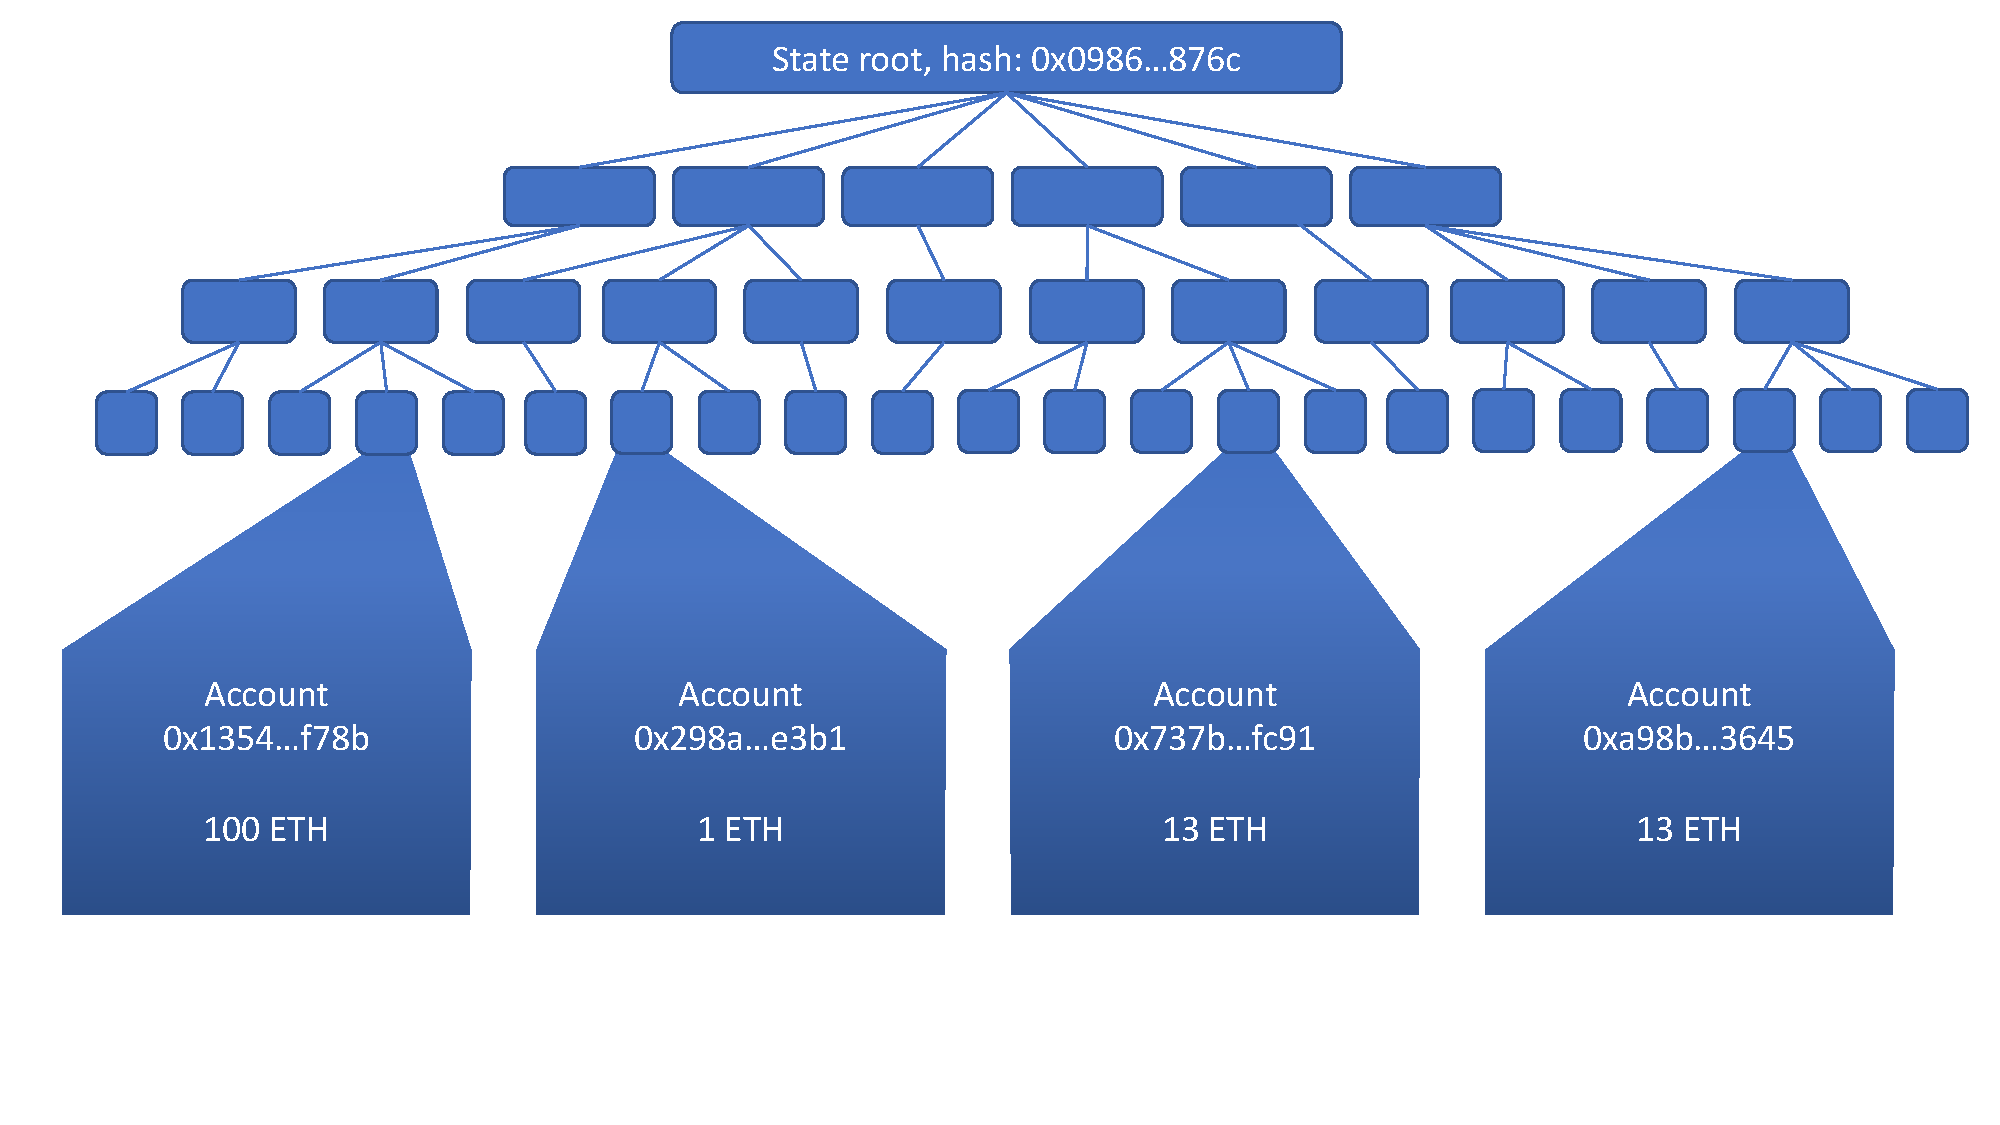
\includegraphics[width=\figurewidth,page=1]{../figures/design/example.pdf}
  \caption{Initial Merkle-Patricia trie. This trie has 22 Ethereum accounts, shown in the last level of the trie. Four accounts are shown in an expanded view. The state root hash is \texttt{0xa34c\ldots 2f55}. The remaining empty nodes are intermediate Merkle-Patricia trie nodes.}
  \label{fig:example:initial}
\end{figure}

Now suppose account \texttt{0x1354\ldots f78b} wants to send 10 ETH to account \texttt{0x298a\ldots e2b1}. This Ethereum transaction is submitted to an Ethereum miner node running the \System implementation. The miner then needs to include this transaction in a block; for simplicity, assume that this is the only transaction the miner will put in the block. The miner needs to perform the following steps, in order:
\begin{enumerate}
  \item Execute the transaction and reward itself with the block reward \emph{locally}, using the miner's local copy of the Ethereum state trie. \label{example:blockcreation:step1}
  \item Obtain Merkle proofs for all values in the state trie that were accessed in step~\ref{example:blockcreation:step1}.
  \item Create a block header, and set the \emph{state root} field to the expected state root of the state trie after executing the transaction and applying the block reward from step~\ref{example:blockcreation:step1}.
  \item Obtain a nonce for the block that satisfies the Proof-Of-Work condition, and set the \emph{nonce} field of the block header.
  \item Send block to other peers.
\end{enumerate}

The miner first needs to execute the transaction with its local copy of the state trie. While it executes the transaction, it keeps track of which accounts in the state trie were accessed. It then constructs Merkle proofs for all accounts that were accessed. After the transaction has been executed, the miner also needs to calculate the block reward. Recall from Section~\ref{subsection:consensus} that miners receive a reward for mining blocks. Suppose the miner's Ethereum address is \texttt{0x737b\ldots fc91} and the block reward is $5$ ETH. The miner also needs to obtain a witness for adding the block reward to its own address. Figure~\ref{fig:example:proof} shows the witnesses generated while creating the block; there are witnesses for accounts \texttt{0x1354\ldots f78b}, \texttt{0x298a\ldots e2b1}, and \texttt{0x737b\ldots fc91}. The state trie after executing the transaction and applying the block reward is shown in Figure~\ref{fig:example:newstate}.

\begin{figure}[H]
  \centering
  \includegraphics[width=\figurewidth,page=3]{../figures/design/example.pdf}
  \caption{The same Merkle-Patricia trie from Figure~\ref{fig:example:initial}, but the nodes in green are the Merkle proofs for the accounts accessed.}
  \label{fig:example:proof}
\end{figure}

\begin{figure}[H]
  \centering
  \includegraphics[width=\figurewidth,page=4]{../figures/design/example.pdf}
  \caption{The updated Merkle-Patricia trie. Note that the balances for the accounts have been changed, and the state root hash is different from the state root hash in Figure~\ref{fig:example:initial}.}
  \label{fig:example:newstate}
\end{figure}

After the witness is generated, the miner needs to create a block header. This block header contains many fields for block metadata, but most importantly for this example, it contains a field for the expected \emph{state root} after the execution of the block. This new state root was calculated earlier when executing the transaction and applying the block reward and is shown in Figure~\ref{fig:example:newstate}. Once the block header is created, the miner can serialize and hash it in order to begin the process of obtaining a nonce for this block for Proof-Of-Work consensus. The \emph{nonce} field in the header is set to the nonce that was found.

After the nonce is obtained, the block is broadcast to other Ethereum nodes. The witnesses are serialized and added to the end of the block, as shown in Figure~\ref{fig:example:block}.

\begin{figure}[H]
  \centering
  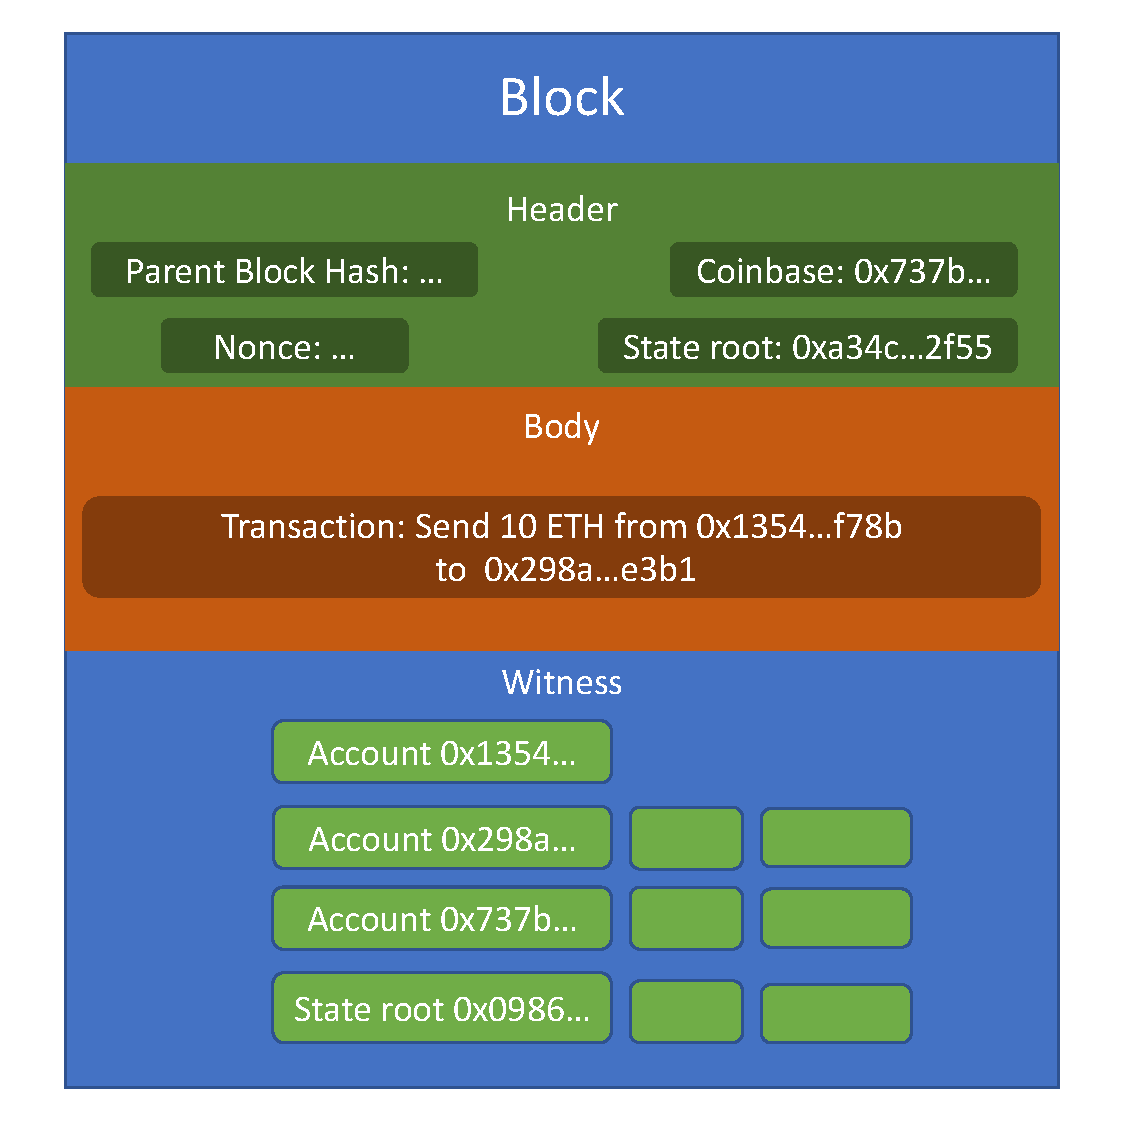
\includegraphics[width=\figurewidth]{../figures/design/example_block.pdf}
  \caption{The newly created block. The Merkle-Patricia nodes in the witnesses are serialized and added to the end of the block. The \emph{coinbase} field in the block header is set to the miner's account address.}
  \label{fig:example:block}
\end{figure}

\subsubsection{Block verification}

\emph{Verifiers} are nodes that do not create blocks and only receive blocks from other peers to verify them. Verifiers are also known as \emph{full nodes}. In \System, verifiers do not store the Ethereum state trie, but they still store the blocks they receive. A verifier node running the \System implementation needs to perform the following steps in order to verify blocks:

\begin{enumerate}
  \item Receive block from peer.
  \item Use witness in block to reconstruct the Merkle-Patricia trie.
  \item Use the \emph{parent block hash} from the block header to find the previous block in the blockchain.
  \item Extract the \emph{state root} field from the header of the previous block. This is the initial state root for the current block.
  \item Execute transaction and apply block reward using the reconstructed Merkle-Patricia trie.
\end{enumerate}

Block verification in \System starts by first receiving a block with witnesses from a miner (Figure~\ref{fig:example:block}). The verifier then reconstructs the Merkle-Patricia state trie using the witnesses in the block. It deserializes the nodes and inserts them into a \texttt{HashMap}, where the key for each node is the SHA-3 hash of the node. Recall from Section~\ref{subsection:merklepatriciatrie} that nodes in a Merkle-Patricia trie link to other nodes using their SHA-3 hash. \texttt{HashMap}s make looking up nodes by their hash efficient. Hashing each node also implicitly verifies the witness, since a malformed witness would have incorrect hashes and the trie would not be able to be reconstructed completely.

To determine which node is the root of the trie, the verifier uses the \emph{parent block hash} to look up the block header of the previous block. The previous block's header contains a \emph{state root} field, which is the state root for the current block. The reconstructed trie is shown in Figure~\ref{fig:example:reconstructed}.

\begin{figure}[H]
  \centering
  \includegraphics[width=\figurewidth,page=5]{../figures/design/example.pdf}
  \caption{The Merkle-Patricia trie reconstructed from the witness in the block.}
  \label{fig:example:reconstructed}
\end{figure}

The verifier then executes the transaction and applies the block reward, using the reconstructed state trie to get account balances. If the transaction execution or block execution tries to access a trie node that is not in the reconstructed trie, then the witness in the block is malformed and the block is not valid. After executing the transaction and the block reward, there is a new state trie with a new state root as shown in Figure~\ref{fig:example:newconstructed}.

\begin{figure}[H]
  \centering
  \includegraphics[width=\figurewidth,page=6]{../figures/design/example.pdf}
  \caption{The updated reconstructed Merkle-Patricia trie. Note that the account balances and the state root hash have changed. The state root hash matches the expected state root hash in the block header in Figure~\ref{fig:example:block}.}
  \label{fig:example:newconstructed}
\end{figure}


\section{Implementation}

I implemented \System in Parity, a popular Ethereum client written in the Rust programming language. The implementation was divided into several logical parts.

\subsection{State backend}


Ethereum state in Parity is accessed through a \texttt{State} struct. \texttt{State} handles the following tasks:
\begin{enumerate}
  \item Create recoverable checkpoints.
  \item Create and retrieve smart contracts.
  \item Create and retrieve account data.
  \item Transfer balances between accounts.
\end{enumerate}

In addition to these tasks, \texttt{State} also maintains an internal cache of the accounts that were requested. Modifications to these accounts are cached and are written to the underlying storage only when the \texttt{State} object is destroyed.

The \texttt{State} struct provides a convenient wrapper around the Ethereum state trie. Other parts of Parity, such as the Ethereum Virtual Machine, use the functions exposed by \texttt{State} to execute transactions. However, the Ethereum state data is not stored inside the \texttt{State} object. \texttt{State} is a generic struct that uses a state backend (a \texttt{Backend} object) to read and write state data.

\texttt{Backend} is a Rust trait. Traits in Rust are similar to interfaces in other languages like Java. Structs that implement the \texttt{Backend} trait need to have the methods defined in Figure~\ref{fig:backendmethods}.

\begin{figure}[H]
  \centering
  \begin{enumerate}
    \item \texttt{Get(key)}
    \item \texttt{Insert(value)}
    \item \texttt{Emplace(key, value)}
    \item \texttt{Contains(key)}
    \item \texttt{Remove(key)}
  \end{enumerate}
  \caption{Required methods for \texttt{Backend}}
  \label{fig:backendmethods}
\end{figure}


The ``standard'' backend that Parity uses is the \texttt{StateDB} backend. \texttt{StateDB} is a struct that contains a pointer to a RocksDB database object and implements each of the required methods by reading and writing from RocksDB. RocksDB is a popular key-value store that Parity uses to store the state trie. The key for each value in the state database is simply the SHA-3 hash of the value.

\begin{figure}[H]
  \centering
  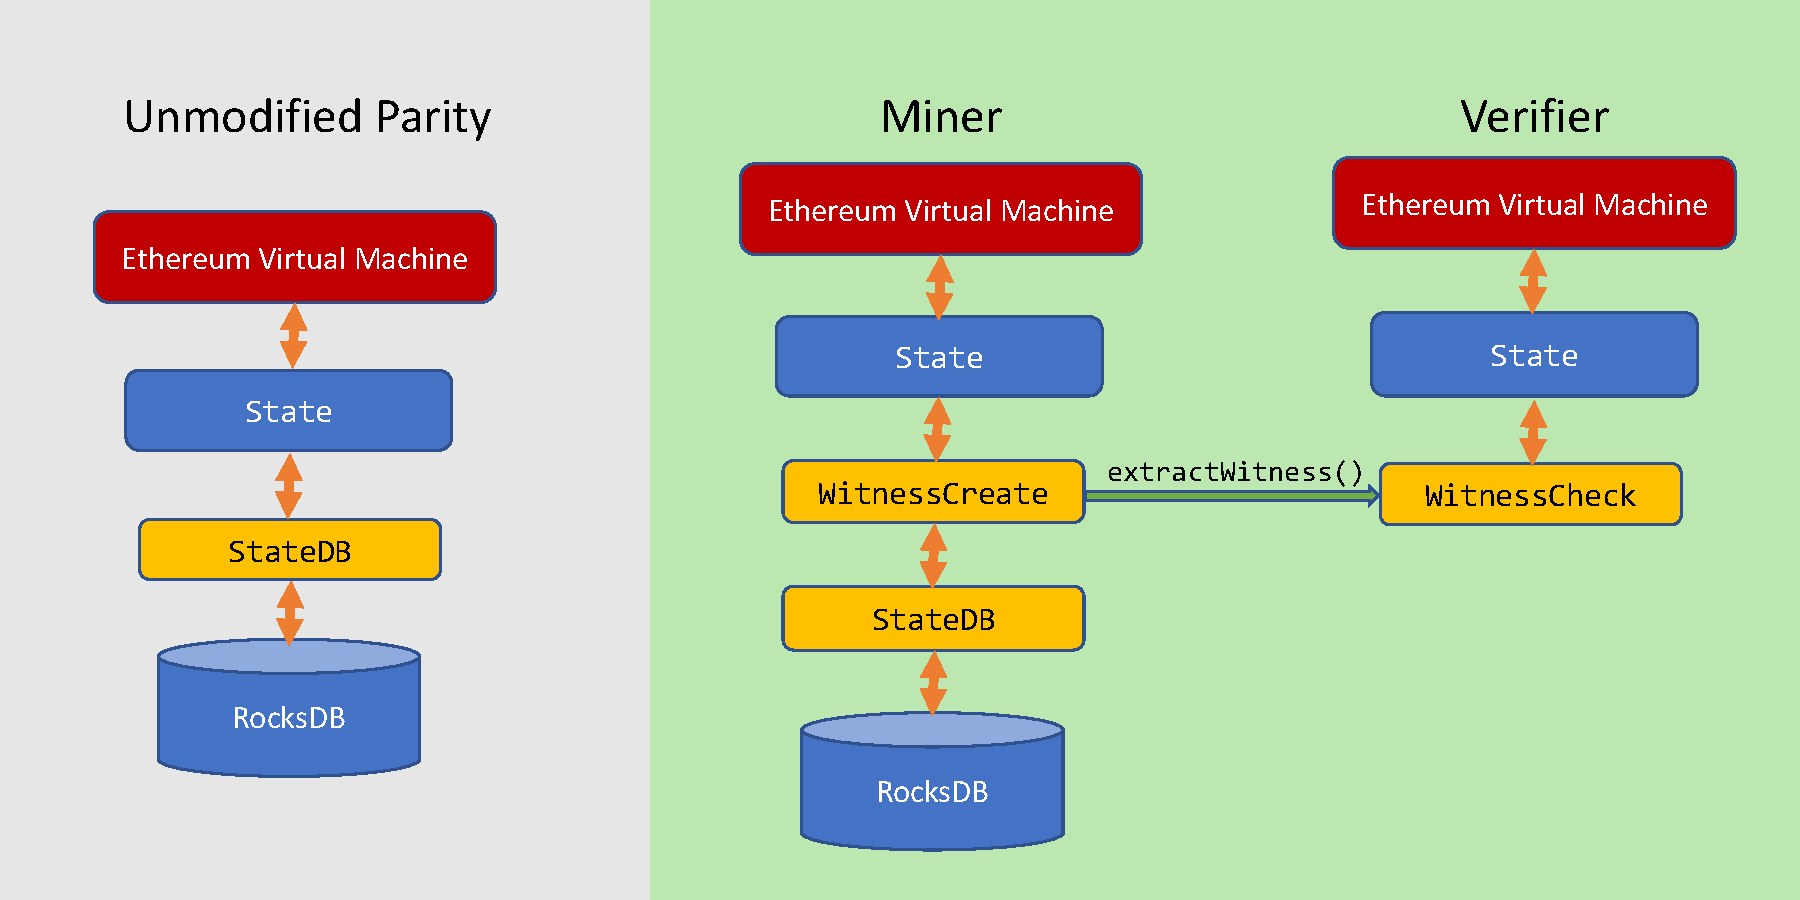
\includegraphics[width=\figurewidth]{../figures/implementation/code_layout.pdf}
  \caption{The relationships between structs in Parity. In unmodified Parity, \texttt{State} communicates with \texttt{StateDB} which uses an on-disk RocksDB key-value store. In the \System implementation, miners have a different code path than verifiers. Miners use \texttt{WitnessCreate} to generate witnesses by intercepting \texttt{Get()} calls to \texttt{StateDB}. Witnesses are extracted from \texttt{WitnessCreate} with \texttt{extractWitnesses()}. Verifiers use \texttt{WitnessCheck} to check these witnesses and use them as a state store for executing transactions.}
  \label{fig:parityrelationships}
\end{figure}

\subsubsection{Witness Creation}

In Parity, blocks are created by a \texttt{Miner} object. Since the \texttt{Miner} object executes transactions, it needs access to the Ethereum state, provided by a \texttt{State} object and a \texttt{Backend} object. I replaced the \texttt{StateDB} backend that the \texttt{Miner} uses with a backend I created called \texttt{WitnessCreate}. The \texttt{WitnessCreate} backend \emph{intercepts} \texttt{Get(key)} and \texttt{Contains(key)} calls and records the values retrieved from the state database. The rest of the methods required for the \texttt{Backend} trait are implemented the same as in \texttt{StateDB}. After all transactions have been executed, the values recorded by \texttt{WitnessCreate} are extracted with a function called \texttt{extractWitness}. This witness is broadcast to the Ethereum network along with the block data once the miner successfully mines the block.

\subsubsection{Witness Verification}

Block verification in Parity has several phases:
\begin{enumerate}
  \item \texttt{verify\_block\_basic}: Checks block integrity, header parameter integrity, and verifies seals for the block and uncles
  \item \texttt{verify\_block\_unordered}: Checks transaction signatures and block nonce
  \item \texttt{verify\_block\_family}: Check block information against parent and uncle blocks.
  \item \texttt{verify\_block\_external}: Consensus engine-specific validation.
  \item \texttt{verify\_block\_final}: Executes the transactions in the block, and checks block information against block execution results. This step makes sure the resulting state root, gas used, log bloom filter, and receipts root match what is recorded in the block header.
\end{enumerate}

I modified the final step of the block verification process to use a \texttt{WitnessCheck} state backend instead of \texttt{StateDB}. When constructing the \texttt{WitnessCheck}, I use the witness that is broadcast with the block (Figure~\ref{fig:parityrelationships}). The \texttt{WitnessCheck} backend implements the methods in Figure~\ref{fig:backendmethods} by using this witness. \texttt{Insert(value)} and \texttt{Emplace(key, value)} are implemented by using an in-memory \texttt{HashMap} to record all write operations to the \texttt{WitnessCheck} backend. \texttt{Get(key)} is implemented by looking for values in the witness that have a SHA-3 hash equal to the \texttt{key}. If no values exist, then the in-memory \texttt{HashMap} is checked. This handles the case when a new value is written and later read from during transaction execution. \texttt{Contains(key)} is implemented by using the same logic as \texttt{Get(key)}, and \texttt{Remove(key)} only removes values from the in-memory \texttt{HashMap} leaving the witness data untouched. There are no read or write operations to the RocksDB state database when verifying blocks.

\subsection{Serialization of witnesses}
An RLP serialized block has the following layout:
\begin{enumerate}
  \item Header
  \begin{enumerate}
    \item Parent block hash
    \item Uncle block hash
    \item Block author
    \item State root hash
    \item Transaction root hash
    \item Block receipts root hash
    \item Log bloom filter
    \item Block difficulty
    \item Block number
    \item Gas limit
    \item Gas used
    \item Timestamp
    \item Extra data
  \end{enumerate}
  \item Body
  \begin{enumerate}
    \item Merkle-Patricia trie of serialized transactions
    \item Merkle-Patricia trie of headers of uncle blocks
    \item \emph{Serialized witness}
  \end{enumerate}
\end{enumerate}

I added an additional field in the \emph{Body} section of the serialized block to store the serialized block witness. The block witness is a list of database values, which can be serialized easily with RLP. The new serialized block format is used when storing blocks on disk, and when syncing blocks over the network. Adding a new field in this location maintains backwards compatibility with unmodified versions of Ethereum.

\subsection{Block sync protocol}

The block sync protocol in Ethereum also needed to be changed. Ethereum nodes use a peer-to-peer (P2P) transport protocol called RLPx~\cite{rlpx} to communicate between nodes. The Ethereum Wire Protocol~\cite{ethereum-wire-protocol} runs on top of RLPx and is used to synchronize the following data among nodes:
\begin{enumerate}
  \item Transactions: When a node receives a transaction, it also broadcasts the same transaction to its peers.
  \item Blocks: When a node mines a new block or receives a new block from a peer, it broadcasts the same block to its peers.
  \item State: Nodes may also synchronize their state tries by broadcasting Merkle tree nodes.
\end{enumerate}


\begin{figure}[H]
  \begin{protocol}{Ethereum block synchronization protocol}
    \emph{Inputs.} Peer $P_1$ contains blocks $B_K = \set{b_{1}, b_{2}, b_{3}, \ldots, b_{K}}$, the set of blocks up to block number $K$. Peer $P_2$ contains blocks $B_H = \set{b_{1}, b_{2}, b_{3}, \ldots, b_{H}}$, the set of blocks up to block number $H$ where $H < K$.
    \sbline
    \emph{Goal.} Peer $P_2$ contains the set of blocks $B_K$.
    \sbline
    \emph{Steps:}
    \begin{enumerate}
      \item $P_1$ and $P_2$ send a \textsc{Status(currentBlockNumber)} message to each other.
      \item $P_2$ notices that its latest block number $H$ is less than $P_1$'s latest block number $K$. $P_2$ sends \textsc{GetBlockHeaders($\set{b_{H+1}, \ldots, b_{K}}$)} to request block headers for blocks $b_{H + 1}, \ldots, b_{K}$ from $P_1$. \label{syncprotocol:requestBlockHeaders}
      \item $P_1$ replies with a \textsc{BlockHeaders} message, containing a list of block headers that $P_2$ requeested. \label{syncprotocol:replyBlockHeaders}
      \item $P_2$ sends \textsc{GetBlockBodies($\setc{b_{H+1}, \ldots, b_{K}}{\text{$b_i$ is not an empty block}}$)} to $P_1$ to request \emph{block bodies}, which are parts of the blocks excluding the header. \label{syncprotocol:requestBlockBodies}
      \item $P_1$ replies with a \textsc{BlockBodies} message, containing a list of block bodies blocks that $P_2$ requested. \label{syncprotocol:replyBlockBodies}
      \item $P_2$ matches block bodies with the block headers it received earlier using root hashes of the transaction and uncle block tries. The matched blocks form $b_{H + 1}, \ldots, b_{K}$ and are stored in $P_2$'s block chain. \label{syncprotocol:reconstruct}
    \end{enumerate}
  \end{protocol}
  \caption{Ethereum block sync protocol.} \label{syncprotocol}
\end{figure}


The block synchronization protocol flow in unmodified Ethereum is described in Figure~\ref{syncprotocol}. First, peers send a \textsc{Status} message to each other. The \textsc{Status} message notifies all participants of the latest block number present in every node. Nodes that need more blocks can request blocks from the node with a greater latest block number. The key part of the sync protocol is that blocks are split into \emph{headers} and \emph{bodies} that are sent separately. First, block headers are requested and sent (step~\ref{syncprotocol:requestBlockHeaders}). Then, in step~\ref{syncprotocol:requestBlockBodies}, block bodies are requested for \emph{non-empty} blocks. A block is \emph{empty} if the block body contains no transactions or uncle block headers. Nodes are able to tell if blocks are empty by reading the block header. If a block is empty, then there is no need to request and send an empty body.


This protocol cannot be used for \System without modifications. The reason is that no block in \System is ``empty'', each block at least contains a witness for the block. Even if a block contains no transactions or uncle blocks, it still updates the Ethereum world state because the miner of the block gets rewarded. Rewarding the miner is done by increasing the balance in the miner's account, and the Ethereum node needs to have a Merkle proof of the current balance of the miner's account.

The modifications that were made to this protocol are the following:
\begin{enumerate}
  \item In step~\ref{syncprotocol:requestBlockBodies}, peers request block bodies for \emph{all} block headers, even if the block header represents a block with no transactions or uncle blocks.
  \item In step~\ref{syncprotocol:replyBlockBodies}, peers that send block bodies also send the witness and the hash of the state root for each block body. The witness is not used in the sync protocol but is used to reconstruct each block from its header and block body in step~\ref{syncprotocol:reconstruct}. The state root is used to match block bodies with block headers in step~\ref{syncprotocol:reconstruct}. The root hashes of the transaction trie and uncle block trie cannot be used for matching because empty blocks share the same hashes for these tries. The state root hash of a block is unique, even for empty blocks, so it may be used to match headers with block bodies.
\end{enumerate}


\section{Evaluation}

\subsection{Correctness}

I tested my implementation of \System for correctness by sending blocks from one instance of Parity to another. The first instance of Parity downloaded blocks from the real Ethereum blockchain and calculated the witness for the block. It then sent the modified block to the second instance of Parity, which was running with the stateless client modifications.

The stateless client Parity instance executed each block using the provided witness for any operations involving the Ethereum state. The stateless client is only able to verify blocks with the witness correctly if the state root hash after executing the transactions within the block matches the state root hash calculated by an unmodified Parity instance. I was able to verify that all blocks in the Ethereum blockchain, up to block 7.3 million, are correctly verified by the stateless client.

\subsection{Results} \label{subsection:results}

I tested the \System in a variety of experiments. The purpose of these experiments was to determine if \System is a viable solution to the scalability problems in Ethereum. All experiments were run on a server with an Intel Xeon CPU E3-1220 v5 at 3.0 GHz, 16 GB of RAM, and a 1.2 TB Intel 750 series NVMe SSD.

\subsubsection{Witness Sizes}

The first experiment I ran measured witness sizes. I imported the first 7.3 million blocks from the Ethereum blockchain into the modified Parity Ethereum client and generated witnesses for them.

\begin{figure}[H]
  \centering
  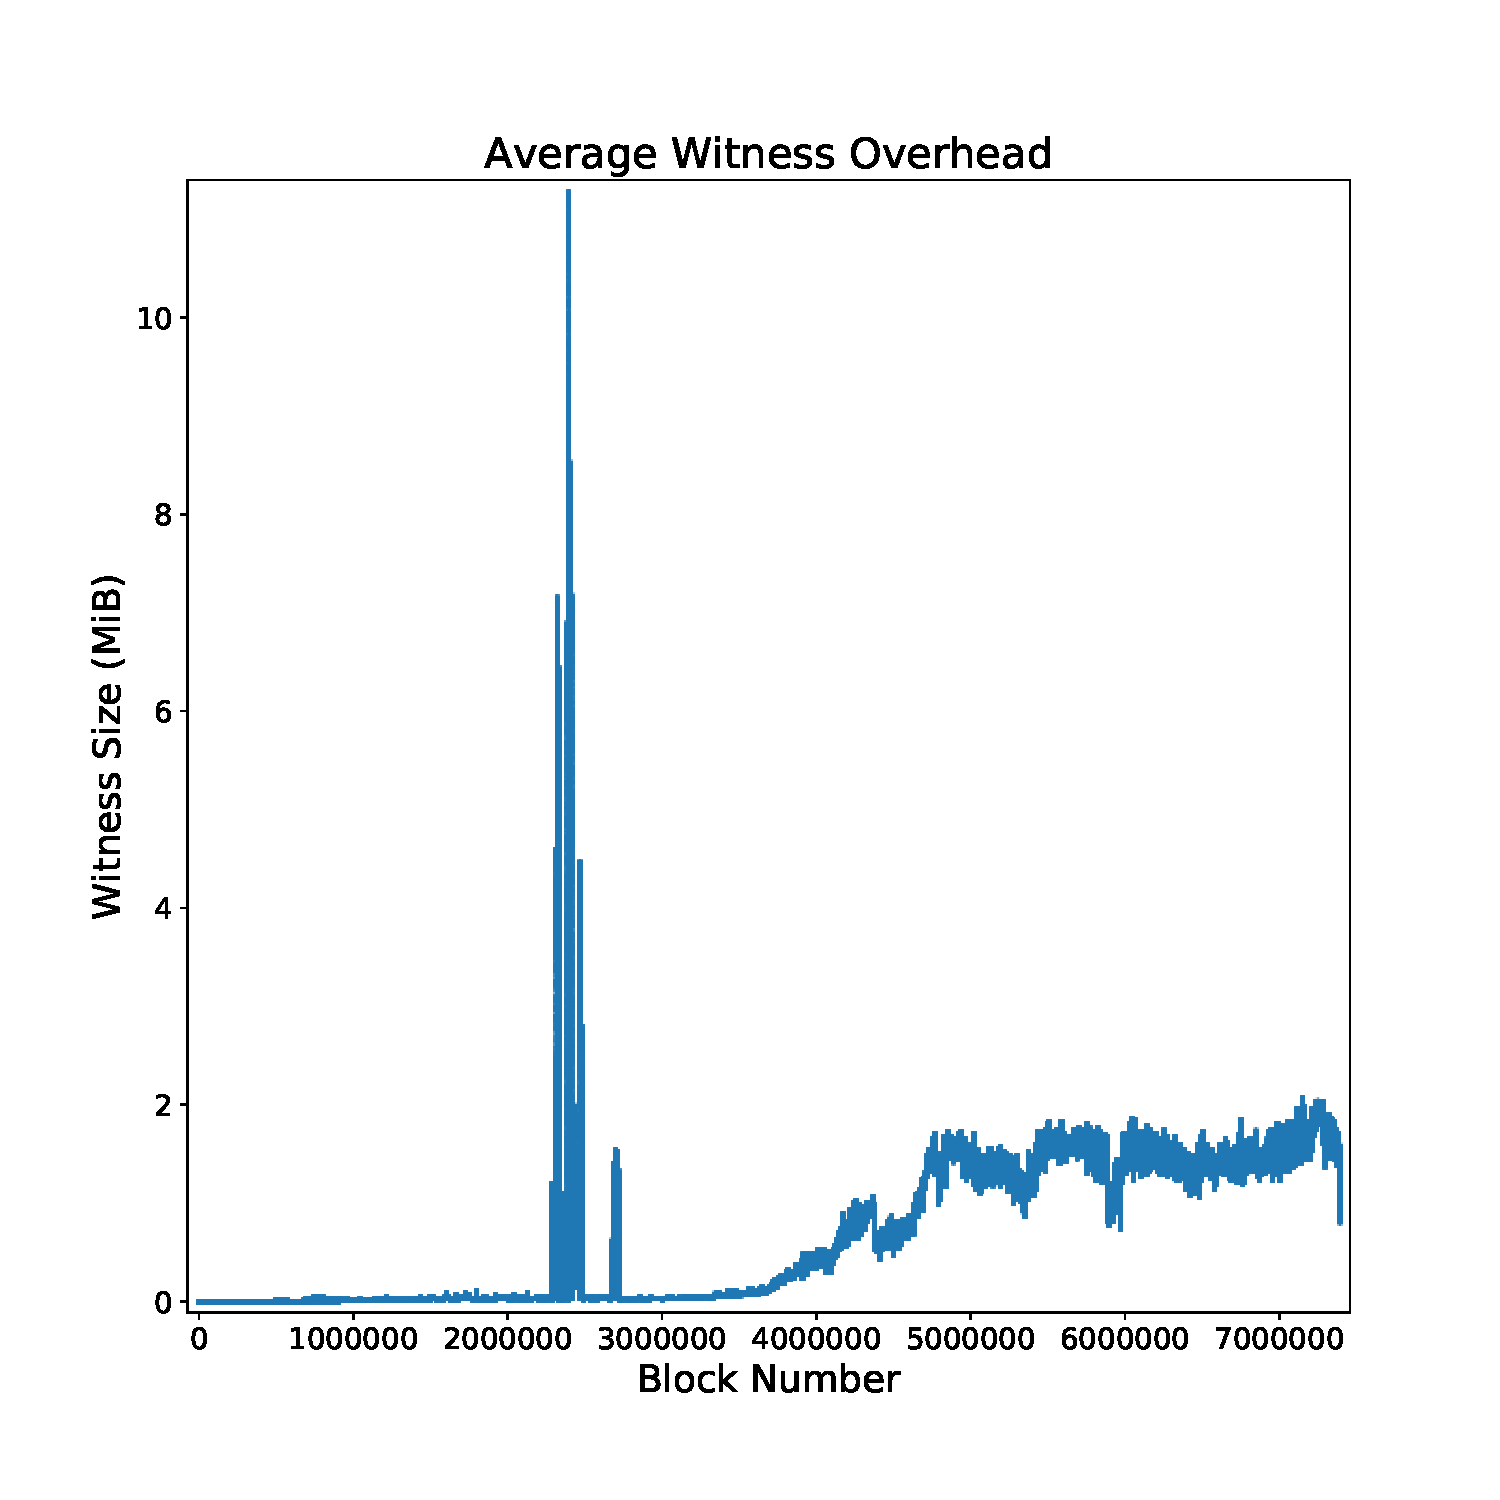
\includegraphics[width=\figurewidth]{../figures/results/graphs/background/witness-size.pdf}
  \caption{Average witness size vs. block number}
  \label{fig:witnesssize}
\end{figure}

Figure~\ref{fig:witnesssize} shows the average witness size per block. The witness size is the total amount in bytes of the RLP serialized witness. There is a lot of variability in witness sizes, so the graph shows a rolling average over the last 2000 blocks at each block number. The average witness size is 723 KB over all blocks. Witness size also generally increases with block number. This is because later blocks tend to contain more transactions than earlier blocks, so more state trie nodes are required for block execution. The size of the state trie also grows as more users create Ethereum accounts, further increasing the witness size. Finally, the increasing frequency of smart contracts that can potentially touch many accounts in a single transaction also contributes to witness size.

The largest witness size was 49.2 MB at block 2306350. The large spikes in the graph from blocks 2.3 to 2.7 million are from a DDoS attack on the Ethereum network in late 2016. This attack created millions of dead Ethereum accounts and significantly increased the size of the state trie. As a result, the witness sizes for blocks in this range are also very large, since they contain millions of newly created accounts.

One important detail to note is that the witness size is \emph{much} larger than the block size excluding the witness. Figure~\ref{fig:blocksize} shows the block sizes excluding the witness, which is the same as the block sizes in unmodified Ethereum. Figure~\ref{fig:witnesssizepct} shows the overhead of including witnesses as a percentage increase over block size excluding witnesses. Witnesses increase block size by about 40x-140x, and the percentage increases with block number.

\begin{figure}[H]
  \centering
  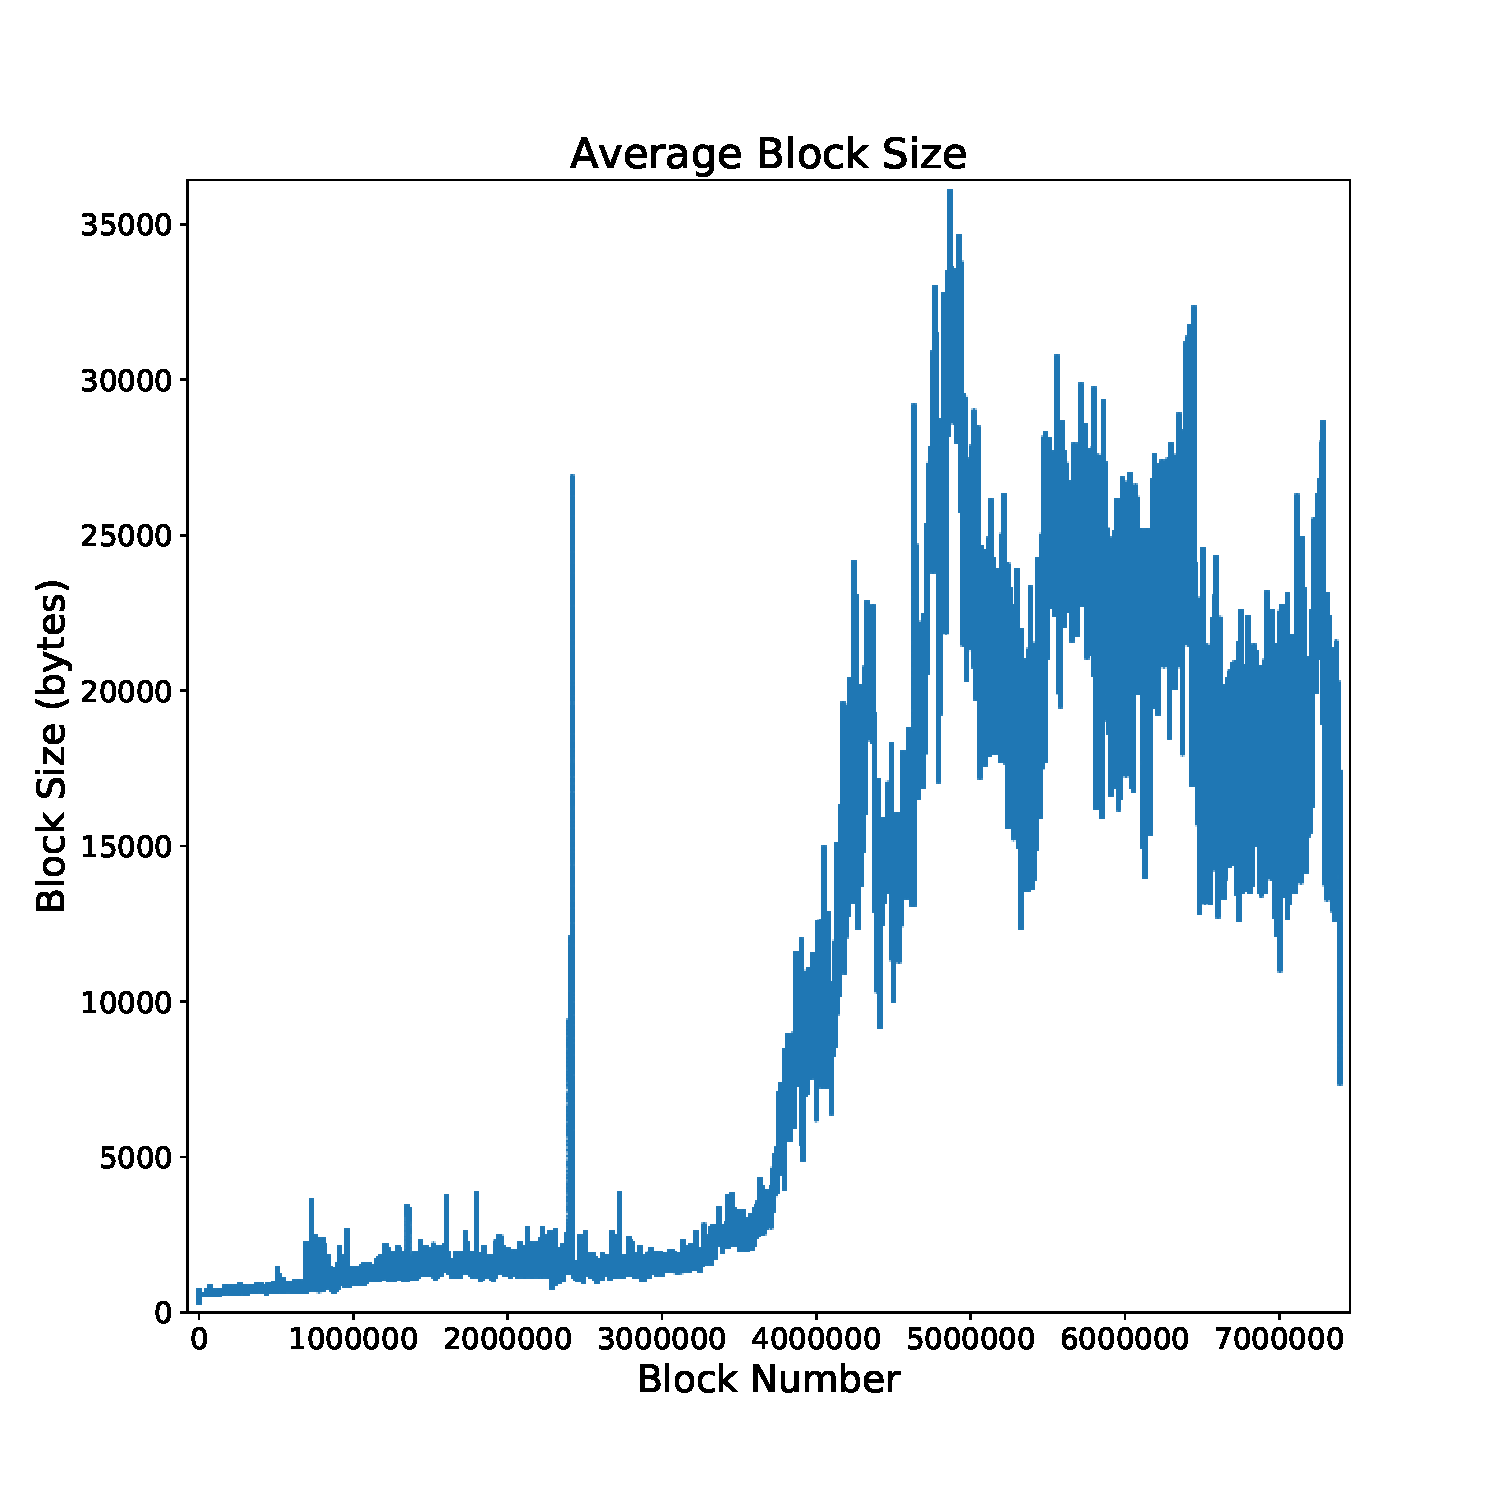
\includegraphics[width=\figurewidth]{../figures/results/graphs/background/block-size.pdf}
  \caption{Average block size (excluding witness) vs. block number}
  \label{fig:blocksize}
\end{figure}

\begin{figure}[H]
  \centering
  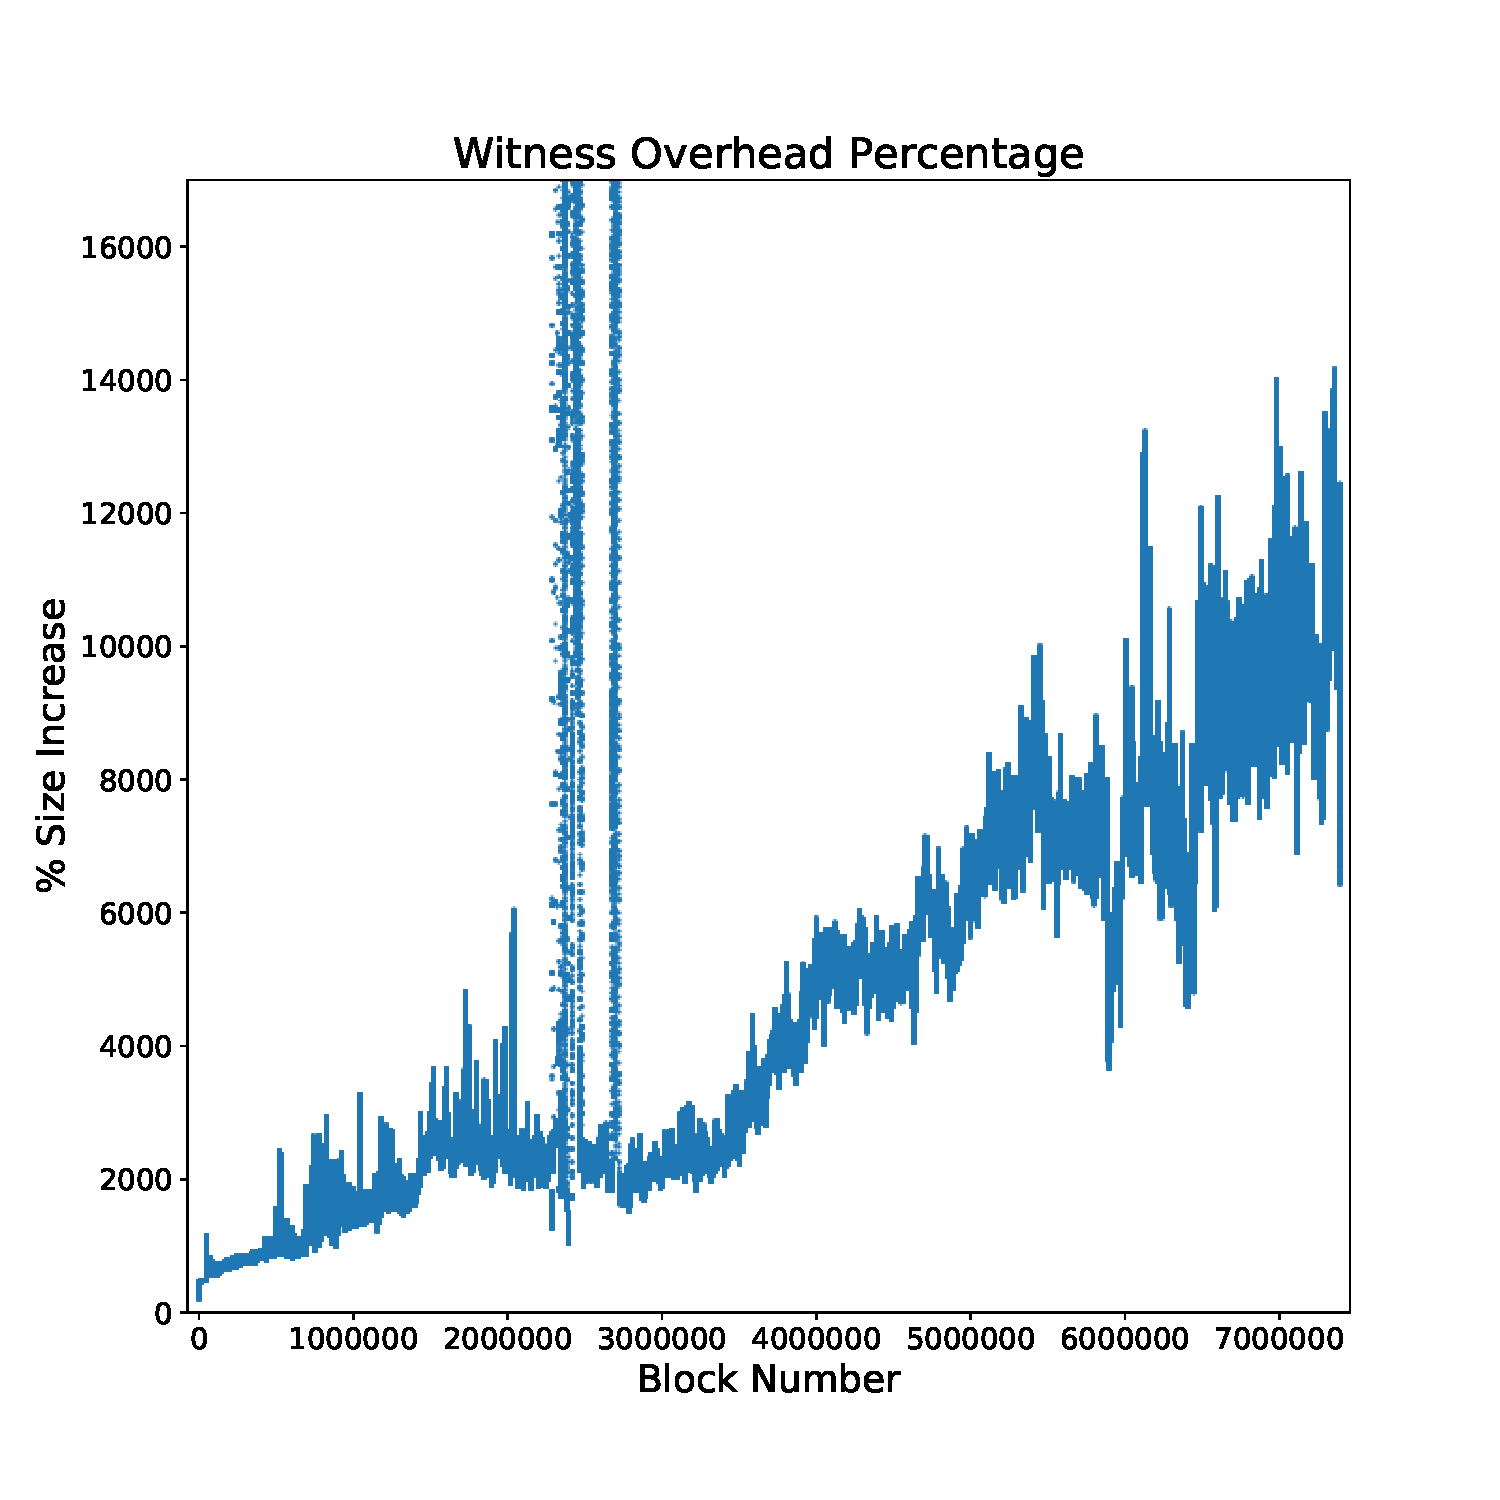
\includegraphics[width=\figurewidth]{../figures/results/graphs/background/witness-block-size.pdf}
  \caption{Average witness size overhead as percentage increase over block size}
  \label{fig:witnesssizepct}
\end{figure}


\subsubsection{Directory Size}

One closely related statistic to witness size is the directory size of the Parity data directory. Parity keeps all data inside a directory specified on the command line with the \texttt{--base-path} argument. This data includes serialized blocks and the state trie, stored in a RocksDB database. I ran a \emph{stateful} Parity node in this experiment. A stateful Parity node uses the same stateless client code, but also maintains its own state trie just as in unmodified Ethereum. Stateful nodes are useful because they act as \emph{translators}; they act as a bridge between the existing Ethereum nodes and stateless nodes by generating witnesses from existing blocks and broadcasting them on the stateless node network. The disk space required for stateful nodes is significantly larger than the space required for an unmodified Parity node, as shown in Figure~\ref{fig:ondisksize}.

\begin{figure}[H]
  \centering
  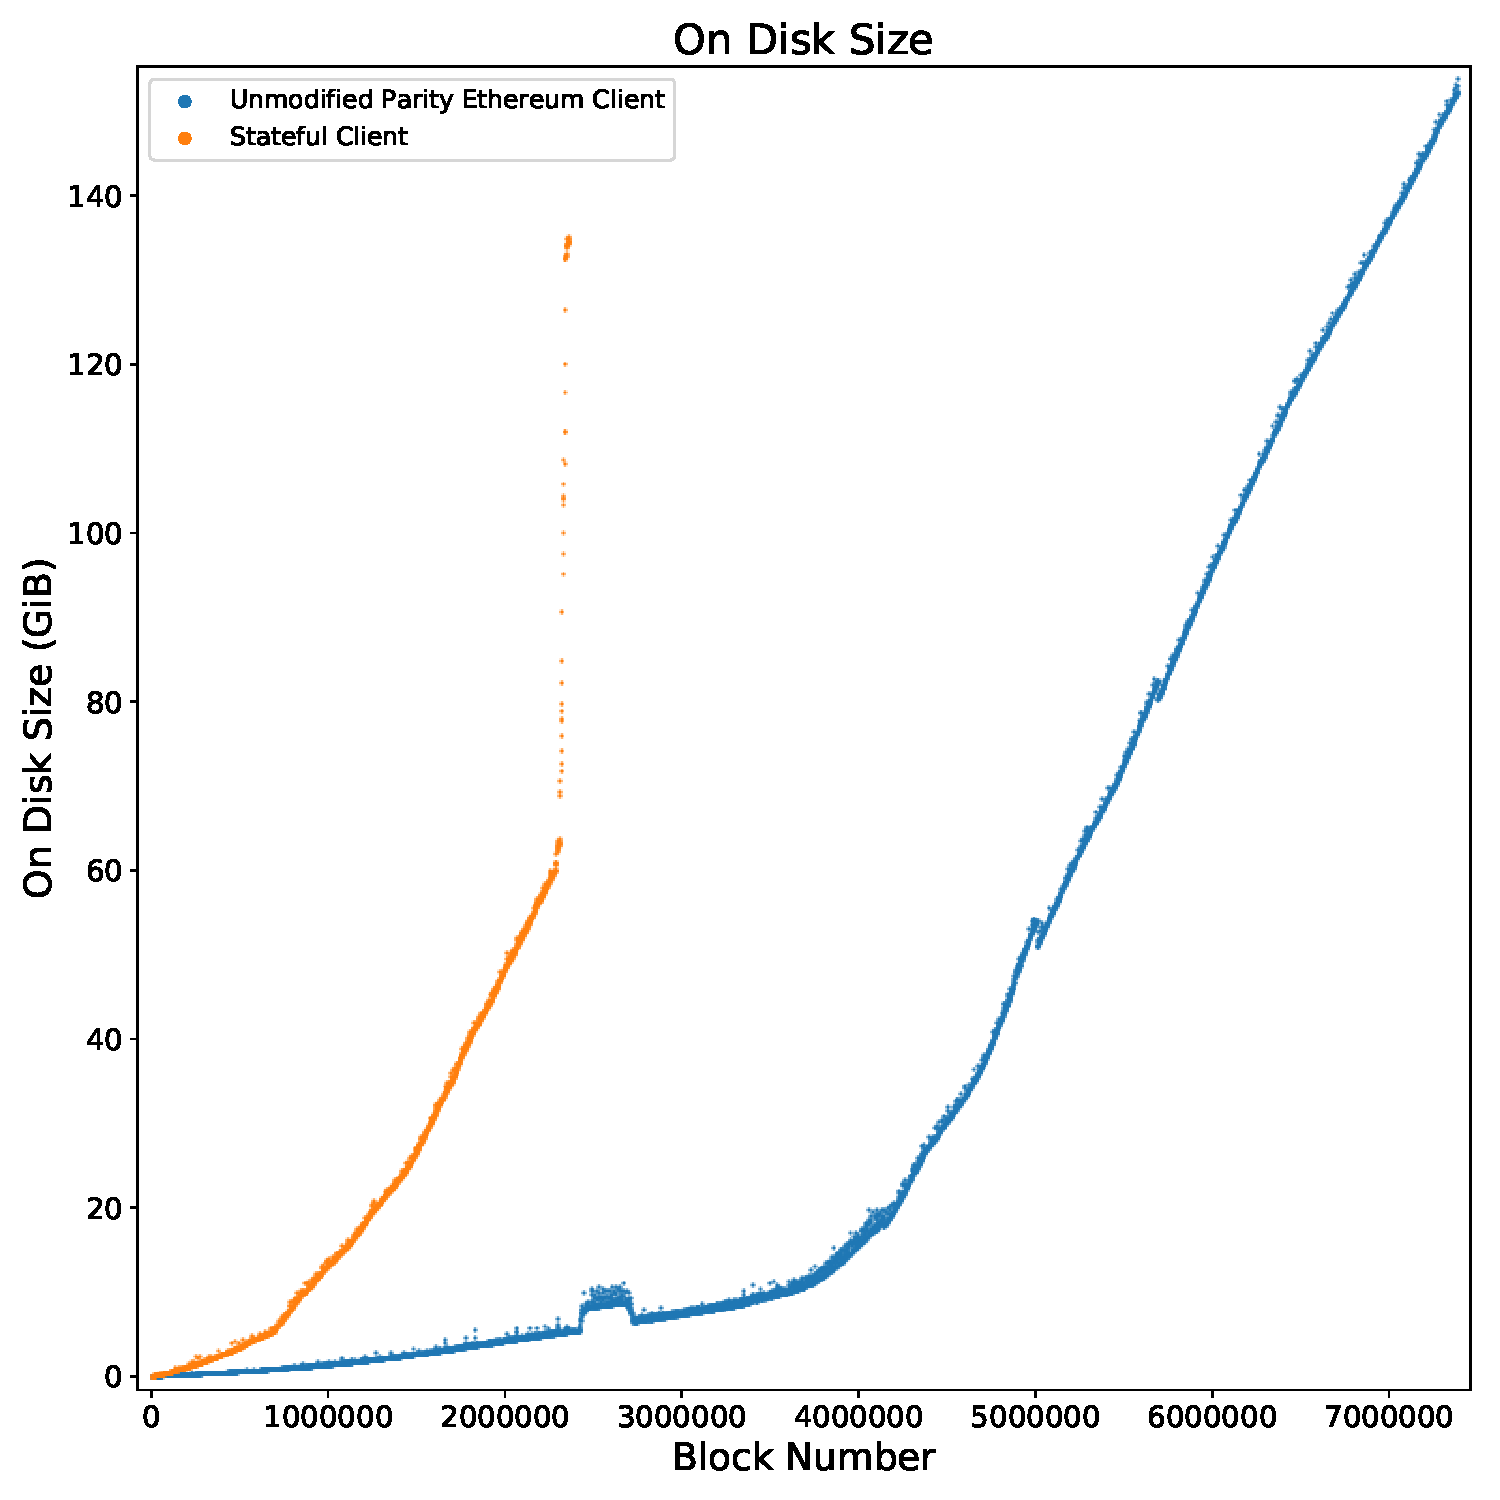
\includegraphics[width=\figurewidth]{../figures/results/graphs/background/on-disk-size.pdf}
  \caption{On-disk size of stateful client and unmodified client vs. block number.}
  \label{fig:ondisksize}
\end{figure}

The disk space required for running a stateful client grows much more quickly than for running an unmodified Parity client. Due to space constraints, I was only able to collect disk usage data for the stateful client only for the first 2.3 million blocks. However, using the data from Figures~\ref{fig:witnesssize}~and~\ref{fig:blocksize}, we are able to project what the on-disk size would be if the experiment had continued.

\begin{figure}[H]
  \centering
  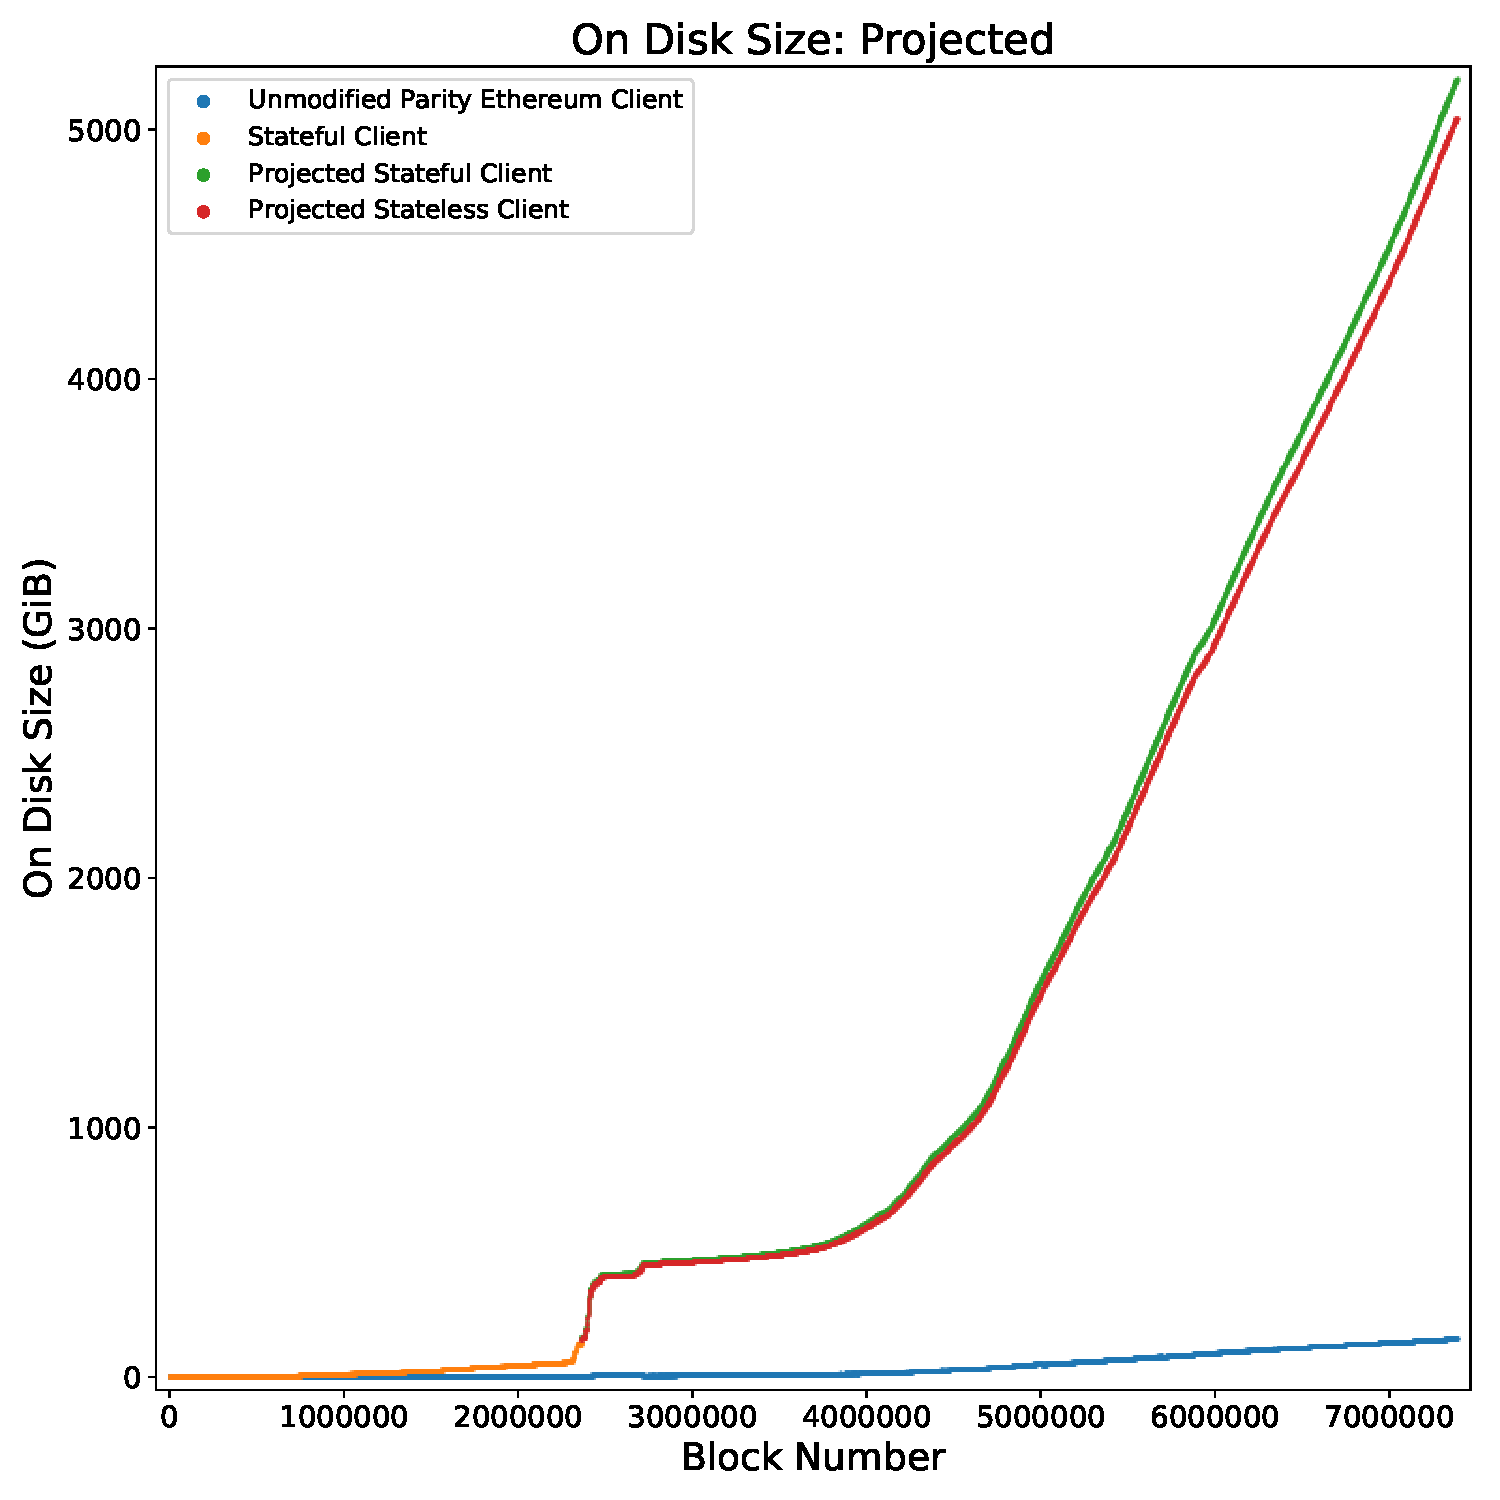
\includegraphics[width=\figurewidth]{../figures/results/graphs/background/projected-on-disk-size.pdf}
  \caption{Projected on-disk size of stateful client and stateless client, compared to actual on-disk size of unmodified client.}
  \label{fig:projectedondisksize}
\end{figure}

The projected data in Figure~\ref{fig:projectedondisksize} was obtained by using cumulative sums of block size and witness size, since the stateful client needs to store the block with its witness locally. If this experiment had continued, then the actual disk usage would be slightly less than the projected usage. This is because RocksDB compresses blockchain data. However, even with the projected data, it is clear that the space required to store witnesses for each block makes the \System proposal impractical. Currently, a new Ethereum block is mined every 15 seconds~\cite{ethereumblocktime}. Using the projected rate of disk usage growth, 1.7 MB of data will have to be stored per new block, amounting to 9.8 GB of additional disk usage per day.

\subsubsection{Database Operations}

One advantage of \System is that the number of database operations is greatly reduced. The only database operations that need to be performed when verifying a block are the following:
\begin{enumerate}
  \item One \textsc{Read} operation to check if the block has already been verified.
  \item One \textsc{Read} operation to check the epoch transition (Section~\ref{subsection:consensus}). This operation is not strictly necessary, and with further optimization this may be removed.
  \item One \textsc{Read} operation to verify each uncle block.
  \item One \textsc{Write} operation to store the new block data.
\end{enumerate}

This is a significant reduction in I/O over the unmodified Parity client, which is shown in Figure~\ref{fig:blockverification}.

\begin{figure}[H]
  \centering
  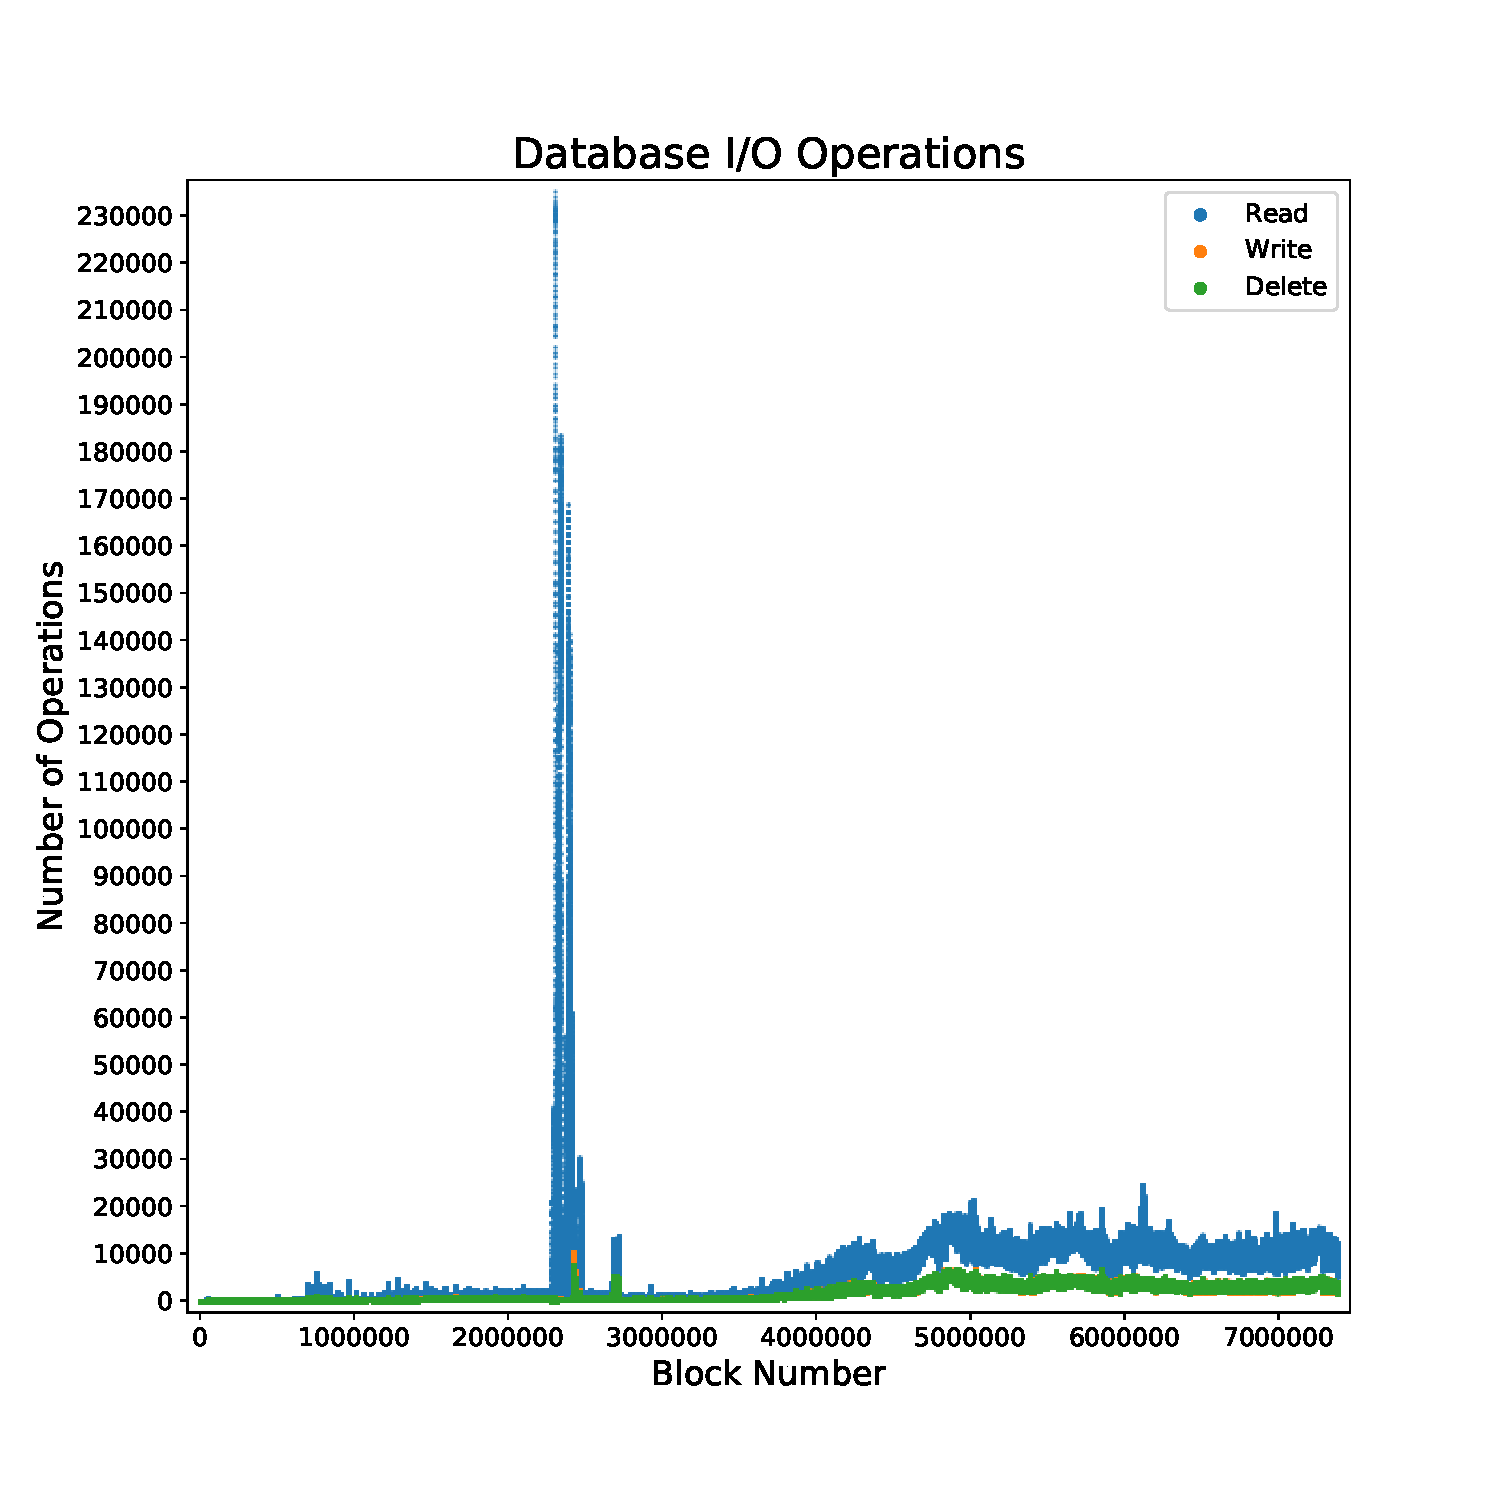
\includegraphics[width=\figurewidth]{../figures/results/graphs/background/db-io-ops.pdf}
  \repeatcaption{fig:blockverification}{I/O operations performed during block verification}
\end{figure}


\subsubsection{Block Import \& Verification Throughput} \label{subsubsection:verificationtime}

\System reduces I/O by bundling witnesses into blocks, but this does not necessarily translate to faster block verification times. I tested this by importing the first 2.3 million blocks along with witnesses into an unmodified Parity instance and Parity with the \system implementation. The 2.3 million blocks were serialized with RLP and stored in a file on-disk. Importing blocks in Parity involves reading each block from disk and verifying the block, using the same verification logic as when receiving blocks over the network from other Ethereum nodes. However, importing blocks from a file removes variability due to network conditions. The rate at which blocks were imported is shown in Figure~\ref{fig:throughput}.

\begin{figure}[H]
  \centering
  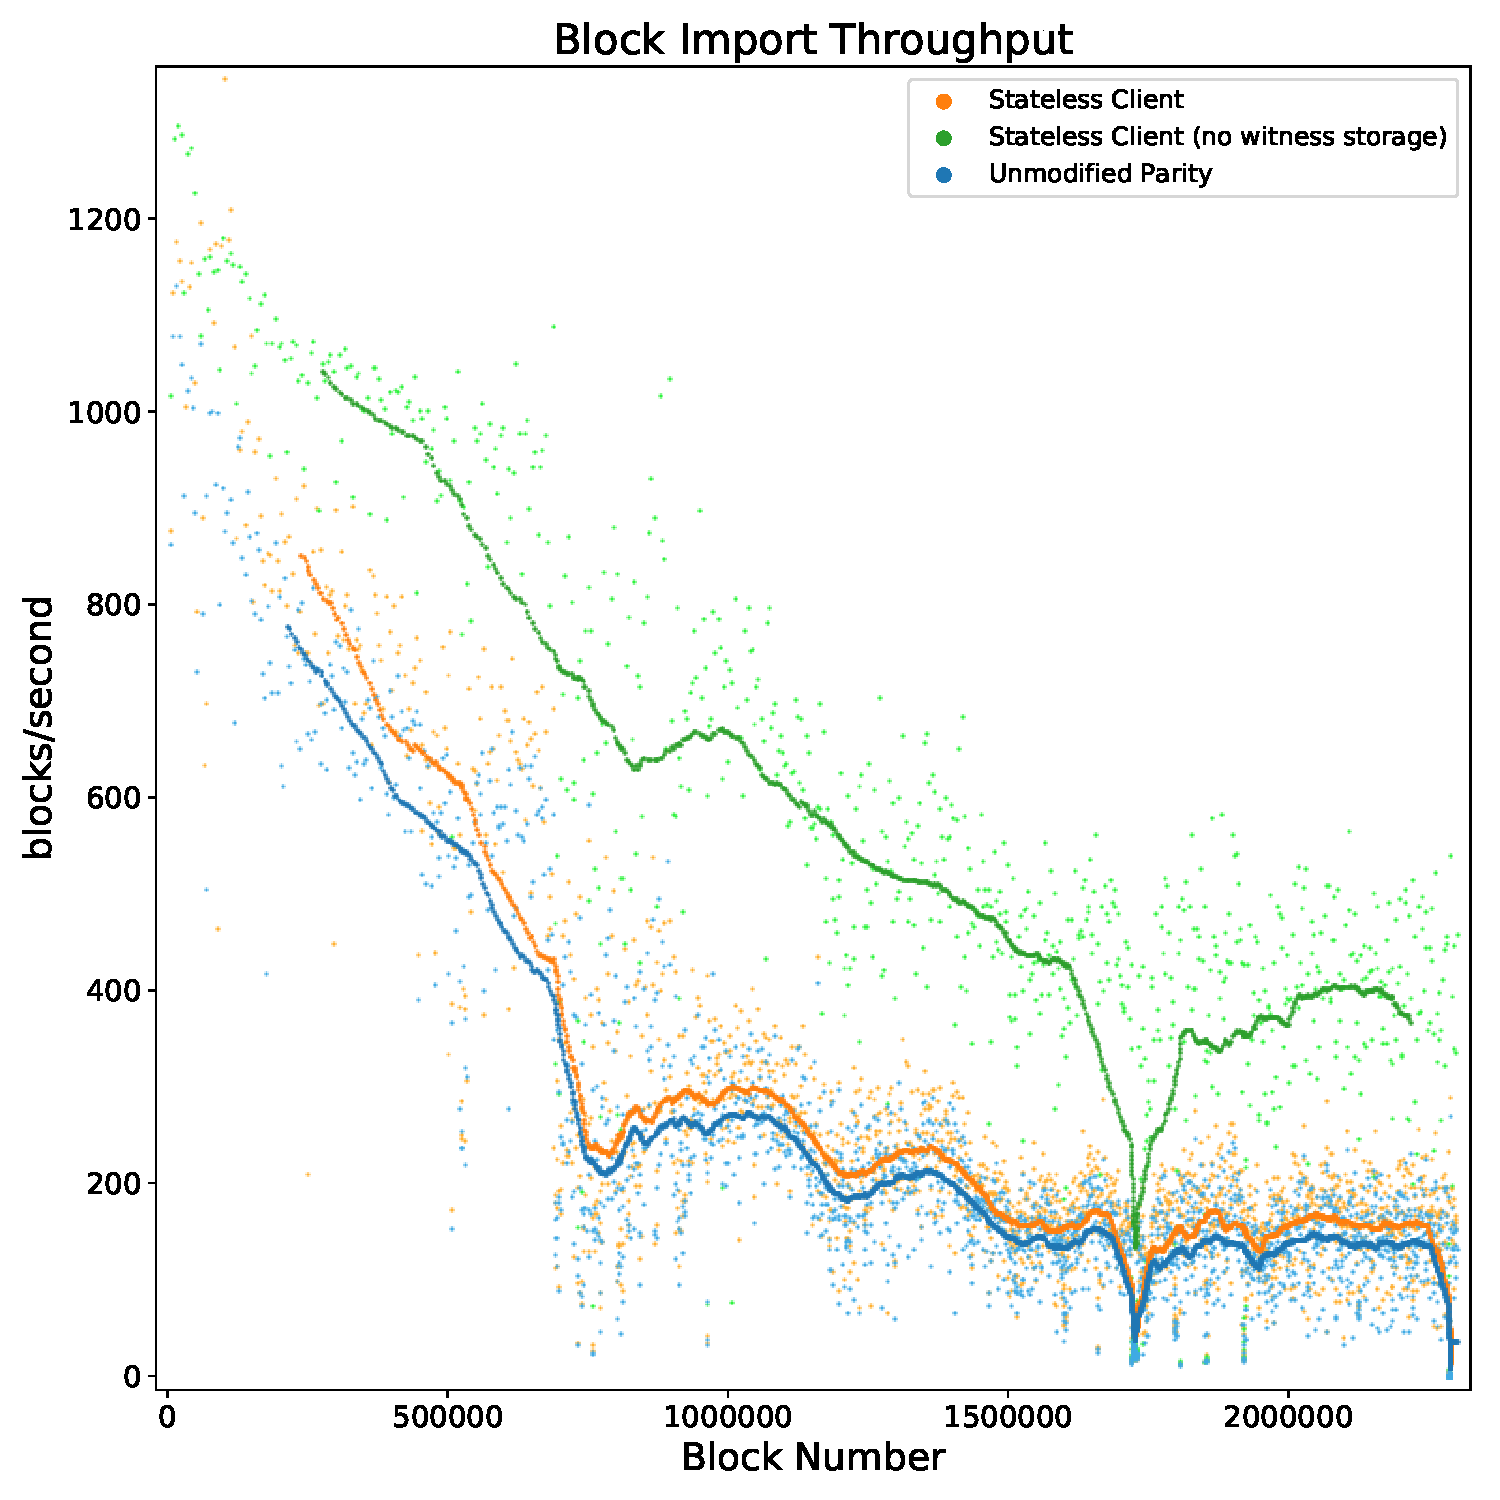
\includegraphics[width=\figurewidth]{../figures/results/graphs/background/throughput.pdf}
  \caption{Block import throughput of unmodified Parity and Parity with \System modifications. The solid lines show a moving average over the last 100 data points. \System performs on average 10\% faster than unmodified Parity.}
  \label{fig:throughput}
\end{figure}

Although \System reduces I/O, the rate at which blocks can be verified is not greatly increased. Parity with \System modifications is only about 10\% faster than unmodified Parity in this benchmark. Using profiling data, I found that a large portion of the execution time spent in the stateless client is inside the SHA-3 hash function. Reconstructing the Merkle-Patricia trie from the block witness is expensive due to the large number of SHA-3 hash calculations required. To make this faster, one solution would be to encode the SHA-3 hash of each node in each Merkle proof in the witness along with the node data. However, this would further increase the witness size.


\section{Related Work}

There are several other potential solutions to scaling blockchains.

\subsection{Ethereum 2.0 Sharding} \label{subsection:ethereumsharding}


\System is part of a larger effort within the Ethereum community to develop \emph{Ethereum 2.0}. Ethereum 2.0 is a set of specifications for the next version of Ethereum. One of the ideas proposed in Ethereum 2.0 is to \emph{shard} the blockchain across multiple collections of nodes~\cite{ethereum-sharding}. Currently, all Ethereum nodes process all transactions. Once a block is mined, it is broadcast to the whole network and every Ethereum node verifies the block independently. The problem with this approach is that the throughput of the entire system is limited by the throughput of a single node.

Ethereum 2.0 Sharding proposes to split the blockchain and state trie into partitions called \emph{``shards''}. One sharding scheme is to create shards based on account addresses. For example, all account addresses starting with \texttt{0x0...} would be in one shard, all account addresses starting with \texttt{0x1...} would be in another shard, and so on until account addresses starting with \texttt{0xf...}. This scheme creates 16 shards, one for each hexadecimal digit from \texttt{0x0} to \texttt{0xf}. Every Ethereum node belongs to a shard and serves requests for that shard. Within a shard, Ethereum transactions are the same as in the current version of Ethereum. However, transactions that access accounts in different shards need to use a complex protocol involving transaction receipts~\cite{ethereum-cross-shard}.


\subsection{Hyperledger Fabric}

Hyperledger Fabric~\cite{androulaki2018hyperledger} is a blockchain architecture that improves scalability in the \emph{permissioned} setting. In contrast to \emph{permissionless} blockchains like Ethereum, peers in permissioned blockchains are not completely untrusted. Hyperledger Fabric improves the performance of permissioned blockchains by using an \emph{execute-order-validate} architecture.
\begin{enumerate}
  \item \emph{Execute:} Executing transactions and checking its correctness (\emph{endorsing}).
  \item \emph{Order:} Use a consensus protocol to order transactions and batch them into blocks.
  \item \emph{Validate:} Validate transactions in blocks.
\end{enumerate}

There are three components to this architecture: \emph{clients}, \emph{peers}, and \emph{orderers}. In the execute step, clients send transactions to peers that execute them and reply back with the execution results. Then, clients send the transactions along with the execution results to the orderers, which use a consensus protocol to order the transactions and package them into blocks. Finally, peers receive these blocks and validate them.

This is similar to \System in that clients do not have access to the blockchain state. Clients submit transactions to peers for execution. This works because in the permissioned setting, the peers are not completely untrusted.

\section{Future Work}

One area that could be explored in the future is different techniques for reducing witness size. In Section~\ref{subsection:results}, I showed how the witness sizes make the \System proposal impractical to use. Reducing witness sizes would not only make \System feasible in terms of network and disk space constraints, but it would also increase block verification throughput (Section~\ref{subsubsection:verificationtime}) due to fewer Merkle-Patricia nodes to read from the witness section of the block data.

There are several techniques for reducing witness size that could be implemented~\cite{ethereum-stateless-analysis}. One technique is to ``cache'' frequently used Merkle-Patricia trie nodes in verifier nodes. Nodes in the first few rows of the Merkle-Patricia trie are referenced often and can be stored locally at the verifier nodes. Then, witnesses no longer need to include full Merkle proofs of state values; they would only need to include Merkle-Patricia trie nodes that are not cached at the verifiers.

Another area that could be explored is implementing Ethereum 2.0 Sharding (Section~\ref{subsection:ethereumsharding}) and determining whether it increases block verification throughput. This would require measuring the throughput of both intra-shard and inter-shard transaction verification to compare against unmodified Ethereum and \System. Exploring the execute-order-verify architecture of Hyperledger Fabric and adapting it to Ethereum is also an area of interest.


\section{Conclusion}

In this project, I worked on implementing the \System proposal in Parity, a popular Ethereum client. The goal of \System is to improve the scalability of Ethereum by reducing I/O operations required to verify blocks. \System does this by bundling a \emph{witness} along with each block, where the witness contains \emph{Merkle proofs} of all the values accessed in the Ethereum state trie during execution of the block. Miners generate witnesses when creating blocks by keeping track of the values accessed during block execution. Verifiers check witnesses for validity and reconstruct Merkle trees in order to verify blocks.

\System does accomplish the goal of reducing I/O operations needed to verify blocks, but the extremely large witness overhead in each block makes using \System impractical. The witness size can be $40-100\times$ the size of the block without witnesses. Reducing witness size and exploring alternate architectures such as Ethereum 2.0 Sharding and the execute-order-verify architecture of Hyperledger Fabric are potential future topics for research.

\section{Acknowledgements}

I would like to first thank my advisor Vijay Chidambaram for his guidance and advice over the last two years. His mentorship was extremely valuable not only for this work but for the other projects I have worked on as part of his research group and for developing my skills as a CS researcher. Next, I would like to thank Soujanya Ponnapalli and Aashaka Shah for proposing the initial idea to me, organizing weekly meetings, and helping me understand blockchain concepts. I also want to thank Chris Rossbach for reviewing a draft of this thesis.


\bibliography{\jobname}
\bibliographystyle{plain}

\end{document}

% Local Variables:
% TeX-command-default: "LatexMk"
% End:
